\documentclass{report}

%%%%%%%%%%%%%%%%%%%%%%%%%%%%%%%%%
% PACKAGE IMPORTS
%%%%%%%%%%%%%%%%%%%%%%%%%%%%%%%%%


\usepackage[tmargin=2cm,rmargin=1in,lmargin=1in,margin=0.85in,bmargin=2cm,footskip=.2in]{geometry}
\usepackage{amsmath,amsfonts,amsthm,amssymb,mathtools}
\usepackage[varbb]{newpxmath}
\usepackage{xfrac}
\usepackage[makeroom]{cancel}
\usepackage{mathtools}
\usepackage{bookmark}
\usepackage{enumitem}
\usepackage{hyperref,theoremref}
\hypersetup{
	pdftitle={Assignment},
	colorlinks=true, linkcolor=doc!90,
	bookmarksnumbered=true,
	bookmarksopen=true
}
\usepackage[most,many,breakable]{tcolorbox}
\usepackage{xcolor}
\usepackage{varwidth}
\usepackage{varwidth}
\usepackage{etoolbox}
%\usepackage{authblk}
\usepackage{nameref}
\usepackage{multicol,array}
\usepackage{tikz-cd}
\usepackage[ruled,vlined,linesnumbered]{algorithm2e}
\usepackage{comment} % enables the use of multi-line comments (\ifx \fi) 
\usepackage{import}
\usepackage{xifthen}
\usepackage{pdfpages}
\usepackage{transparent}

\newcommand\mycommfont[1]{\footnotesize\ttfamily\textcolor{blue}{#1}}
\SetCommentSty{mycommfont}
\newcommand{\incfig}[1]{%
    \def\svgwidth{\columnwidth}
    \import{./figures/}{#1.pdf_tex}
}

\usepackage{tikzsymbols}
\renewcommand\qedsymbol{$\Laughey$}


%\usepackage{import}
%\usepackage{xifthen}
%\usepackage{pdfpages}
%\usepackage{transparent}


%%%%%%%%%%%%%%%%%%%%%%%%%%%%%%
% SELF MADE COLORS
%%%%%%%%%%%%%%%%%%%%%%%%%%%%%%



\definecolor{myg}{RGB}{56, 140, 70}
\definecolor{myb}{RGB}{45, 111, 177}
\definecolor{myr}{RGB}{199, 68, 64}
\definecolor{mytheorembg}{HTML}{F2F2F9}
\definecolor{mytheoremfr}{HTML}{00007B}
\definecolor{mylenmabg}{HTML}{FFFAF8}
\definecolor{mylenmafr}{HTML}{983b0f}
\definecolor{mypropbg}{HTML}{f2fbfc}
\definecolor{mypropfr}{HTML}{191971}
\definecolor{myexamplebg}{HTML}{F2FBF8}
\definecolor{myexamplefr}{HTML}{88D6D1}
\definecolor{myexampleti}{HTML}{2A7F7F}
\definecolor{mydefinitbg}{HTML}{E5E5FF}
\definecolor{mydefinitfr}{HTML}{3F3FA3}
\definecolor{notesgreen}{RGB}{0,162,0}
\definecolor{myp}{RGB}{197, 92, 212}
\definecolor{mygr}{HTML}{2C3338}
\definecolor{myred}{RGB}{127,0,0}
\definecolor{myyellow}{RGB}{169,121,69}
\definecolor{myexercisebg}{HTML}{F2FBF8}
\definecolor{myexercisefg}{HTML}{88D6D1}


%%%%%%%%%%%%%%%%%%%%%%%%%%%%
% TCOLORBOX SETUPS
%%%%%%%%%%%%%%%%%%%%%%%%%%%%

\setlength{\parindent}{1cm}
%================================
% THEOREM BOX
%================================

\tcbuselibrary{theorems,skins,hooks}
\newtcbtheorem[number within=section]{Theorem}{Theorem}
{%
	enhanced,
	breakable,
	colback = mytheorembg,
	frame hidden,
	boxrule = 0sp,
	borderline west = {2pt}{0pt}{mytheoremfr},
	sharp corners,
	detach title,
	before upper = \tcbtitle\par\smallskip,
	coltitle = mytheoremfr,
	fonttitle = \bfseries\sffamily,
	description font = \mdseries,
	separator sign none,
	segmentation style={solid, mytheoremfr},
}
{th}

\tcbuselibrary{theorems,skins,hooks}
\newtcbtheorem[number within=chapter]{theorem}{Theorem}
{%
	enhanced,
	breakable,
	colback = mytheorembg,
	frame hidden,
	boxrule = 0sp,
	borderline west = {2pt}{0pt}{mytheoremfr},
	sharp corners,
	detach title,
	before upper = \tcbtitle\par\smallskip,
	coltitle = mytheoremfr,
	fonttitle = \bfseries\sffamily,
	description font = \mdseries,
	separator sign none,
	segmentation style={solid, mytheoremfr},
}
{th}


\tcbuselibrary{theorems,skins,hooks}
\newtcolorbox{Theoremcon}
{%
	enhanced
	,breakable
	,colback = mytheorembg
	,frame hidden
	,boxrule = 0sp
	,borderline west = {2pt}{0pt}{mytheoremfr}
	,sharp corners
	,description font = \mdseries
	,separator sign none
}

%================================
% Corollery
%================================
\tcbuselibrary{theorems,skins,hooks}
\newtcbtheorem[number within=section]{Corollary}{Corollary}
{%
	enhanced
	,breakable
	,colback = myp!10
	,frame hidden
	,boxrule = 0sp
	,borderline west = {2pt}{0pt}{myp!85!black}
	,sharp corners
	,detach title
	,before upper = \tcbtitle\par\smallskip
	,coltitle = myp!85!black
	,fonttitle = \bfseries\sffamily
	,description font = \mdseries
	,separator sign none
	,segmentation style={solid, myp!85!black}
}
{th}
\tcbuselibrary{theorems,skins,hooks}
\newtcbtheorem[number within=chapter]{corollary}{Corollary}
{%
	enhanced
	,breakable
	,colback = myp!10
	,frame hidden
	,boxrule = 0sp
	,borderline west = {2pt}{0pt}{myp!85!black}
	,sharp corners
	,detach title
	,before upper = \tcbtitle\par\smallskip
	,coltitle = myp!85!black
	,fonttitle = \bfseries\sffamily
	,description font = \mdseries
	,separator sign none
	,segmentation style={solid, myp!85!black}
}
{th}


%================================
% LENMA
%================================

\tcbuselibrary{theorems,skins,hooks}
\newtcbtheorem[number within=section]{Lenma}{Lenma}
{%
	enhanced,
	breakable,
	colback = mylenmabg,
	frame hidden,
	boxrule = 0sp,
	borderline west = {2pt}{0pt}{mylenmafr},
	sharp corners,
	detach title,
	before upper = \tcbtitle\par\smallskip,
	coltitle = mylenmafr,
	fonttitle = \bfseries\sffamily,
	description font = \mdseries,
	separator sign none,
	segmentation style={solid, mylenmafr},
}
{th}

\tcbuselibrary{theorems,skins,hooks}
\newtcbtheorem[number within=chapter]{lenma}{Lenma}
{%
	enhanced,
	breakable,
	colback = mylenmabg,
	frame hidden,
	boxrule = 0sp,
	borderline west = {2pt}{0pt}{mylenmafr},
	sharp corners,
	detach title,
	before upper = \tcbtitle\par\smallskip,
	coltitle = mylenmafr,
	fonttitle = \bfseries\sffamily,
	description font = \mdseries,
	separator sign none,
	segmentation style={solid, mylenmafr},
}
{th}


%================================
% PROPOSITION
%================================

\tcbuselibrary{theorems,skins,hooks}
\newtcbtheorem[number within=section]{Prop}{Proposition}
{%
	enhanced,
	breakable,
	colback = mypropbg,
	frame hidden,
	boxrule = 0sp,
	borderline west = {2pt}{0pt}{mypropfr},
	sharp corners,
	detach title,
	before upper = \tcbtitle\par\smallskip,
	coltitle = mypropfr,
	fonttitle = \bfseries\sffamily,
	description font = \mdseries,
	separator sign none,
	segmentation style={solid, mypropfr},
}
{th}

\tcbuselibrary{theorems,skins,hooks}
\newtcbtheorem[number within=chapter]{prop}{Proposition}
{%
	enhanced,
	breakable,
	colback = mypropbg,
	frame hidden,
	boxrule = 0sp,
	borderline west = {2pt}{0pt}{mypropfr},
	sharp corners,
	detach title,
	before upper = \tcbtitle\par\smallskip,
	coltitle = mypropfr,
	fonttitle = \bfseries\sffamily,
	description font = \mdseries,
	separator sign none,
	segmentation style={solid, mypropfr},
}
{th}


%================================
% CLAIM
%================================

\tcbuselibrary{theorems,skins,hooks}
\newtcbtheorem[number within=section]{claim}{Claim}
{%
	enhanced
	,breakable
	,colback = myg!10
	,frame hidden
	,boxrule = 0sp
	,borderline west = {2pt}{0pt}{myg}
	,sharp corners
	,detach title
	,before upper = \tcbtitle\par\smallskip
	,coltitle = myg!85!black
	,fonttitle = \bfseries\sffamily
	,description font = \mdseries
	,separator sign none
	,segmentation style={solid, myg!85!black}
}
{th}



%================================
% Exercise
%================================

\tcbuselibrary{theorems,skins,hooks}
\newtcbtheorem[number within=section]{Exercise}{Exercise}
{%
	enhanced,
	breakable,
	colback = myexercisebg,
	frame hidden,
	boxrule = 0sp,
	borderline west = {2pt}{0pt}{myexercisefg},
	sharp corners,
	detach title,
	before upper = \tcbtitle\par\smallskip,
	coltitle = myexercisefg,
	fonttitle = \bfseries\sffamily,
	description font = \mdseries,
	separator sign none,
	segmentation style={solid, myexercisefg},
}
{th}

\tcbuselibrary{theorems,skins,hooks}
\newtcbtheorem[number within=chapter]{exercise}{Exercise}
{%
	enhanced,
	breakable,
	colback = myexercisebg,
	frame hidden,
	boxrule = 0sp,
	borderline west = {2pt}{0pt}{myexercisefg},
	sharp corners,
	detach title,
	before upper = \tcbtitle\par\smallskip,
	coltitle = myexercisefg,
	fonttitle = \bfseries\sffamily,
	description font = \mdseries,
	separator sign none,
	segmentation style={solid, myexercisefg},
}
{th}

%================================
% EXAMPLE BOX
%================================

\newtcbtheorem[number within=section]{Example}{Example}
{%
	colback = myexamplebg
	,breakable
	,colframe = myexamplefr
	,coltitle = myexampleti
	,boxrule = 1pt
	,sharp corners
	,detach title
	,before upper=\tcbtitle\par\smallskip
	,fonttitle = \bfseries
	,description font = \mdseries
	,separator sign none
	,description delimiters parenthesis
}
{ex}

\newtcbtheorem[number within=chapter]{example}{Example}
{%
	colback = myexamplebg
	,breakable
	,colframe = myexamplefr
	,coltitle = myexampleti
	,boxrule = 1pt
	,sharp corners
	,detach title
	,before upper=\tcbtitle\par\smallskip
	,fonttitle = \bfseries
	,description font = \mdseries
	,separator sign none
	,description delimiters parenthesis
}
{ex}

%================================
% DEFINITION BOX
%================================

\newtcbtheorem[number within=section]{Definition}{Definition}{enhanced,
	before skip=2mm,after skip=2mm, colback=red!5,colframe=red!80!black,boxrule=0.5mm,
	attach boxed title to top left={xshift=1cm,yshift*=1mm-\tcboxedtitleheight}, varwidth boxed title*=-3cm,
	boxed title style={frame code={
					\path[fill=tcbcolback]
					([yshift=-1mm,xshift=-1mm]frame.north west)
					arc[start angle=0,end angle=180,radius=1mm]
					([yshift=-1mm,xshift=1mm]frame.north east)
					arc[start angle=180,end angle=0,radius=1mm];
					\path[left color=tcbcolback!60!black,right color=tcbcolback!60!black,
						middle color=tcbcolback!80!black]
					([xshift=-2mm]frame.north west) -- ([xshift=2mm]frame.north east)
					[rounded corners=1mm]-- ([xshift=1mm,yshift=-1mm]frame.north east)
					-- (frame.south east) -- (frame.south west)
					-- ([xshift=-1mm,yshift=-1mm]frame.north west)
					[sharp corners]-- cycle;
				},interior engine=empty,
		},
	fonttitle=\bfseries,
	title={#2},#1}{def}
\newtcbtheorem[number within=chapter]{definition}{Definition}{enhanced,
	before skip=2mm,after skip=2mm, colback=red!5,colframe=red!80!black,boxrule=0.5mm,
	attach boxed title to top left={xshift=1cm,yshift*=1mm-\tcboxedtitleheight}, varwidth boxed title*=-3cm,
	boxed title style={frame code={
					\path[fill=tcbcolback]
					([yshift=-1mm,xshift=-1mm]frame.north west)
					arc[start angle=0,end angle=180,radius=1mm]
					([yshift=-1mm,xshift=1mm]frame.north east)
					arc[start angle=180,end angle=0,radius=1mm];
					\path[left color=tcbcolback!60!black,right color=tcbcolback!60!black,
						middle color=tcbcolback!80!black]
					([xshift=-2mm]frame.north west) -- ([xshift=2mm]frame.north east)
					[rounded corners=1mm]-- ([xshift=1mm,yshift=-1mm]frame.north east)
					-- (frame.south east) -- (frame.south west)
					-- ([xshift=-1mm,yshift=-1mm]frame.north west)
					[sharp corners]-- cycle;
				},interior engine=empty,
		},
	fonttitle=\bfseries,
	title={#2},#1}{def}



%================================
% Solution BOX
%================================

\makeatletter
\newtcbtheorem{question}{Question}{enhanced,
	breakable,
	colback=white,
	colframe=myb!80!black,
	attach boxed title to top left={yshift*=-\tcboxedtitleheight},
	fonttitle=\bfseries,
	title={#2},
	boxed title size=title,
	boxed title style={%
			sharp corners,
			rounded corners=northwest,
			colback=tcbcolframe,
			boxrule=0pt,
		},
	underlay boxed title={%
			\path[fill=tcbcolframe] (title.south west)--(title.south east)
			to[out=0, in=180] ([xshift=5mm]title.east)--
			(title.center-|frame.east)
			[rounded corners=\kvtcb@arc] |-
			(frame.north) -| cycle;
		},
	#1
}{def}
\makeatother

%================================
% SOLUTION BOX
%================================

\makeatletter
\newtcolorbox{solution}{enhanced,
	breakable,
	colback=white,
	colframe=myg!80!black,
	attach boxed title to top left={yshift*=-\tcboxedtitleheight},
	title=Solution,
	boxed title size=title,
	boxed title style={%
			sharp corners,
			rounded corners=northwest,
			colback=tcbcolframe,
			boxrule=0pt,
		},
	underlay boxed title={%
			\path[fill=tcbcolframe] (title.south west)--(title.south east)
			to[out=0, in=180] ([xshift=5mm]title.east)--
			(title.center-|frame.east)
			[rounded corners=\kvtcb@arc] |-
			(frame.north) -| cycle;
		},
}
\makeatother

%================================
% Question BOX
%================================

\makeatletter
\newtcbtheorem{qstion}{Question}{enhanced,
	breakable,
	colback=white,
	colframe=mygr,
	attach boxed title to top left={yshift*=-\tcboxedtitleheight},
	fonttitle=\bfseries,
	title={#2},
	boxed title size=title,
	boxed title style={%
			sharp corners,
			rounded corners=northwest,
			colback=tcbcolframe,
			boxrule=0pt,
		},
	underlay boxed title={%
			\path[fill=tcbcolframe] (title.south west)--(title.south east)
			to[out=0, in=180] ([xshift=5mm]title.east)--
			(title.center-|frame.east)
			[rounded corners=\kvtcb@arc] |-
			(frame.north) -| cycle;
		},
	#1
}{def}
\makeatother

\newtcbtheorem[number within=chapter]{wconc}{Wrong Concept}{
	breakable,
	enhanced,
	colback=white,
	colframe=myr,
	arc=0pt,
	outer arc=0pt,
	fonttitle=\bfseries\sffamily\large,
	colbacktitle=myr,
	attach boxed title to top left={},
	boxed title style={
			enhanced,
			skin=enhancedfirst jigsaw,
			arc=3pt,
			bottom=0pt,
			interior style={fill=myr}
		},
	#1
}{def}



%================================
% NOTE BOX
%================================

\usetikzlibrary{arrows,calc,shadows.blur}
\tcbuselibrary{skins}
\newtcolorbox{note}[1][]{%
	enhanced jigsaw,
	colback=gray!20!white,%
	colframe=gray!80!black,
	size=small,
	boxrule=1pt,
	title=\textbf{Note:-},
	halign title=flush center,
	coltitle=black,
	breakable,
	drop shadow=black!50!white,
	attach boxed title to top left={xshift=1cm,yshift=-\tcboxedtitleheight/2,yshifttext=-\tcboxedtitleheight/2},
	minipage boxed title=1.5cm,
	boxed title style={%
			colback=white,
			size=fbox,
			boxrule=1pt,
			boxsep=2pt,
			underlay={%
					\coordinate (dotA) at ($(interior.west) + (-0.5pt,0)$);
					\coordinate (dotB) at ($(interior.east) + (0.5pt,0)$);
					\begin{scope}
						\clip (interior.north west) rectangle ([xshift=3ex]interior.east);
						\filldraw [white, blur shadow={shadow opacity=60, shadow yshift=-.75ex}, rounded corners=2pt] (interior.north west) rectangle (interior.south east);
					\end{scope}
					\begin{scope}[gray!80!black]
						\fill (dotA) circle (2pt);
						\fill (dotB) circle (2pt);
					\end{scope}
				},
		},
	#1,
}

%%%%%%%%%%%%%%%%%%%%%%%%%%%%%%
% SELF MADE COMMANDS
%%%%%%%%%%%%%%%%%%%%%%%%%%%%%%


\newcommand{\thm}[2]{\begin{Theorem}{#1}{}#2\end{Theorem}}
\newcommand{\cor}[2]{\begin{Corollary}{#1}{}#2\end{Corollary}}
\newcommand{\mlenma}[2]{\begin{Lenma}{#1}{}#2\end{Lenma}}
\newcommand{\mprop}[2]{\begin{Prop}{#1}{}#2\end{Prop}}
\newcommand{\clm}[3]{\begin{claim}{#1}{#2}#3\end{claim}}
\newcommand{\wc}[2]{\begin{wconc}{#1}{}\setlength{\parindent}{1cm}#2\end{wconc}}
\newcommand{\thmcon}[1]{\begin{Theoremcon}{#1}\end{Theoremcon}}
\newcommand{\ex}[2]{\begin{Example}{#1}{}#2\end{Example}}
\newcommand{\dfn}[2]{\begin{Definition}[colbacktitle=red!75!black]{#1}{}#2\end{Definition}}
\newcommand{\dfnc}[2]{\begin{definition}[colbacktitle=red!75!black]{#1}{}#2\end{definition}}
\newcommand{\qs}[2]{\begin{question}{#1}{}#2\end{question}}
\newcommand{\pf}[2]{\begin{myproof}[#1]#2\end{myproof}}
\newcommand{\nt}[1]{\begin{note}#1\end{note}}
\newcommand{\mat}[1]{\begin{bmatrix} #1 \end{bmatrix}}
\newcommand{\vect}[1]{\begin{bmatrix} #1 \end{bmatrix}}

\newcommand*\circled[1]{\tikz[baseline=(char.base)]{
		\node[shape=circle,draw,inner sep=1pt] (char) {#1};}}
\newcommand\getcurrentref[1]{%
	\ifnumequal{\value{#1}}{0}
	{??}
	{\the\value{#1}}%
}
\newcommand{\getCurrentSectionNumber}{\getcurrentref{section}}
\newenvironment{myproof}[1][\proofname]{%
	\proof[\bfseries #1: ]%
}{\endproof}

\newcommand{\mclm}[2]{\begin{myclaim}[#1]#2\end{myclaim}}
\newenvironment{myclaim}[1][\claimname]{\proof[\bfseries #1: ]}{}

\newcounter{mylabelcounter}

\makeatletter
\newcommand{\setword}[2]{%
	\phantomsection
	#1\def\@currentlabel{\unexpanded{#1}}\label{#2}%
}
\makeatother




\tikzset{
	symbol/.style={
			draw=none,
			every to/.append style={
					edge node={node [sloped, allow upside down, auto=false]{$#1$}}}
		}
}


% deliminators
\DeclarePairedDelimiter{\abs}{\lvert}{\rvert}
\DeclarePairedDelimiter{\norm}{\lVert}{\rVert}

\DeclarePairedDelimiter{\ceil}{\lceil}{\rceil}
\DeclarePairedDelimiter{\floor}{\lfloor}{\rfloor}
\DeclarePairedDelimiter{\round}{\lfloor}{\rceil}

\newsavebox\diffdbox
\newcommand{\slantedromand}{{\mathpalette\makesl{d}}}
\newcommand{\makesl}[2]{%
\begingroup
\sbox{\diffdbox}{$\mathsurround=0pt#1\mathrm{#2}$}%
\pdfsave
\pdfsetmatrix{1 0 0.2 1}%
\rlap{\usebox{\diffdbox}}%
\pdfrestore
\hskip\wd\diffdbox
\endgroup
}
\newcommand{\dd}[1][]{\ensuremath{\mathop{}\!\ifstrempty{#1}{%
\slantedromand\@ifnextchar^{\hspace{0.2ex}}{\hspace{0.1ex}}}%
{\slantedromand\hspace{0.2ex}^{#1}}}}
\ProvideDocumentCommand\dv{o m g}{%
  \ensuremath{%
    \IfValueTF{#3}{%
      \IfNoValueTF{#1}{%
        \frac{\dd #2}{\dd #3}%
      }{%
        \frac{\dd^{#1} #2}{\dd #3^{#1}}%
      }%
    }{%
      \IfNoValueTF{#1}{%
        \frac{\dd}{\dd #2}%
      }{%
        \frac{\dd^{#1}}{\dd #2^{#1}}%
      }%
    }%
  }%
}
\providecommand*{\pdv}[3][]{\frac{\partial^{#1}#2}{\partial#3^{#1}}}
%  - others
\DeclareMathOperator{\Lap}{\mathcal{L}}
\DeclareMathOperator{\Var}{Var} % varience
\DeclareMathOperator{\Cov}{Cov} % covarience
\DeclareMathOperator{\E}{E} % expected

% Since the amsthm package isn't loaded

% I prefer the slanted \leq
\let\oldleq\leq % save them in case they're every wanted
\let\oldgeq\geq
\renewcommand{\leq}{\leqslant}
\renewcommand{\geq}{\geqslant}

% % redefine matrix env to allow for alignment, use r as default
% \renewcommand*\env@matrix[1][r]{\hskip -\arraycolsep
%     \let\@ifnextchar\new@ifnextchar
%     \array{*\c@MaxMatrixCols #1}}


%\usepackage{framed}
%\usepackage{titletoc}
%\usepackage{etoolbox}
%\usepackage{lmodern}


%\patchcmd{\tableofcontents}{\contentsname}{\sffamily\contentsname}{}{}

%\renewenvironment{leftbar}
%{\def\FrameCommand{\hspace{6em}%
%		{\color{myyellow}\vrule width 2pt depth 6pt}\hspace{1em}}%
%	\MakeFramed{\parshape 1 0cm \dimexpr\textwidth-6em\relax\FrameRestore}\vskip2pt%
%}
%{\endMakeFramed}

%\titlecontents{chapter}
%[0em]{\vspace*{2\baselineskip}}
%{\parbox{4.5em}{%
%		\hfill\Huge\sffamily\bfseries\color{myred}\thecontentspage}%
%	\vspace*{-2.3\baselineskip}\leftbar\textsc{\small\chaptername~\thecontentslabel}\\\sffamily}
%{}{\endleftbar}
%\titlecontents{section}
%[8.4em]
%{\sffamily\contentslabel{3em}}{}{}
%{\hspace{0.5em}\nobreak\itshape\color{myred}\contentspage}
%\titlecontents{subsection}
%[8.4em]
%{\sffamily\contentslabel{3em}}{}{}  
%{\hspace{0.5em}\nobreak\itshape\color{myred}\contentspage}



%%%%%%%%%%%%%%%%%%%%%%%%%%%%%%%%%%%%%%%%%%%
% TABLE OF CONTENTS
%%%%%%%%%%%%%%%%%%%%%%%%%%%%%%%%%%%%%%%%%%%

\usepackage{tikz}
\definecolor{doc}{RGB}{0,60,110}
\usepackage{titletoc}
\contentsmargin{0cm}
\titlecontents{chapter}[3.7pc]
{\addvspace{30pt}%
	\begin{tikzpicture}[remember picture, overlay]%
		\draw[fill=doc!60,draw=doc!60] (-7,-.1) rectangle (-0.9,.5);%
		\pgftext[left,x=-3.5cm,y=0.2cm]{\color{white}\Large\sc\bfseries Chapter\ \thecontentslabel};%
	\end{tikzpicture}\color{doc!60}\large\sc\bfseries}%
{}
{}
{\;\titlerule\;\large\sc\bfseries Page \thecontentspage
	\begin{tikzpicture}[remember picture, overlay]
		\draw[fill=doc!60,draw=doc!60] (2pt,0) rectangle (4,0.1pt);
	\end{tikzpicture}}%
\titlecontents{section}[3.7pc]
{\addvspace{2pt}}
{\contentslabel[\thecontentslabel]{2pc}}
{}
{\hfill\small \thecontentspage}
[]
\titlecontents*{subsection}[3.7pc]
{\addvspace{-1pt}\small}
{}
{}
{\ --- \small\thecontentspage}
[ \textbullet\ ][]

\makeatletter
\renewcommand{\tableofcontents}{%
	\chapter*{%
	  \vspace*{-20\p@}%
	  \begin{tikzpicture}[remember picture, overlay]%
		  \pgftext[right,x=15cm,y=0.2cm]{\color{doc!60}\Huge\sc\bfseries \contentsname};%
		  \draw[fill=doc!60,draw=doc!60] (13,-.75) rectangle (20,1);%
		  \clip (13,-.75) rectangle (20,1);
		  \pgftext[right,x=15cm,y=0.2cm]{\color{white}\Huge\sc\bfseries \contentsname};%
	  \end{tikzpicture}}%
	\@starttoc{toc}}
\makeatother


%From M275 "Topology" at SJSU
\newcommand{\id}{\mathrm{id}}
\newcommand{\taking}[1]{\xrightarrow{#1}}
\newcommand{\inv}{^{-1}}

%From M170 "Introduction to Graph Theory" at SJSU
\DeclareMathOperator{\diam}{diam}
\DeclareMathOperator{\ord}{ord}
\newcommand{\defeq}{\overset{\mathrm{def}}{=}}

%From the USAMO .tex files
\newcommand{\ts}{\textsuperscript}
\newcommand{\dg}{^\circ}
\newcommand{\ii}{\item}

% % From Math 55 and Math 145 at Harvard
% \newenvironment{subproof}[1][Proof]{%
% \begin{proof}[#1] \renewcommand{\qedsymbol}{$\blacksquare$}}%
% {\end{proof}}

\newcommand{\liff}{\leftrightarrow}
\newcommand{\lthen}{\rightarrow}
\newcommand{\opname}{\operatorname}
\newcommand{\surjto}{\twoheadrightarrow}
\newcommand{\injto}{\hookrightarrow}
\newcommand{\On}{\mathrm{On}} % ordinals
\DeclareMathOperator{\img}{im} % Image
\DeclareMathOperator{\Img}{Im} % Image
\DeclareMathOperator{\coker}{coker} % Cokernel
\DeclareMathOperator{\Coker}{Coker} % Cokernel
\DeclareMathOperator{\Ker}{Ker} % Kernel
\DeclareMathOperator{\rank}{rank}
\DeclareMathOperator{\Spec}{Spec} % spectrum
\DeclareMathOperator{\Tr}{Tr} % trace
\DeclareMathOperator{\pr}{pr} % projection
\DeclareMathOperator{\ext}{ext} % extension
\DeclareMathOperator{\pred}{pred} % predecessor
\DeclareMathOperator{\dom}{dom} % domain
\DeclareMathOperator{\ran}{ran} % range
\DeclareMathOperator{\Hom}{Hom} % homomorphism
\DeclareMathOperator{\Mor}{Mor} % morphisms
\DeclareMathOperator{\End}{End} % endomorphism

\newcommand{\eps}{\epsilon}
\newcommand{\veps}{\varepsilon}
\newcommand{\ol}{\overline}
\newcommand{\ul}{\underline}
\newcommand{\wt}{\widetilde}
\newcommand{\wh}{\widehat}
\newcommand{\vocab}[1]{\textbf{\color{blue} #1}}
\providecommand{\half}{\frac{1}{2}}
\newcommand{\dang}{\measuredangle} %% Directed angle
\newcommand{\ray}[1]{\overrightarrow{#1}}
\newcommand{\seg}[1]{\overline{#1}}
\newcommand{\arc}[1]{\wideparen{#1}}
\DeclareMathOperator{\cis}{cis}
\DeclareMathOperator*{\lcm}{lcm}
\DeclareMathOperator*{\argmin}{arg min}
\DeclareMathOperator*{\argmax}{arg max}
\newcommand{\cycsum}{\sum_{\mathrm{cyc}}}
\newcommand{\symsum}{\sum_{\mathrm{sym}}}
\newcommand{\cycprod}{\prod_{\mathrm{cyc}}}
\newcommand{\symprod}{\prod_{\mathrm{sym}}}
\newcommand{\Qed}{\begin{flushright}\qed\end{flushright}}
\newcommand{\parinn}{\setlength{\parindent}{1cm}}
\newcommand{\parinf}{\setlength{\parindent}{0cm}}
% \newcommand{\norm}{\|\cdot\|}
\newcommand{\inorm}{\norm_{\infty}}
\newcommand{\opensets}{\{V_{\alpha}\}_{\alpha\in I}}
\newcommand{\oset}{V_{\alpha}}
\newcommand{\opset}[1]{V_{\alpha_{#1}}}
\newcommand{\lub}{\text{lub}}
\newcommand{\del}[2]{\frac{\partial #1}{\partial #2}}
\newcommand{\Del}[3]{\frac{\partial^{#1} #2}{\partial^{#1} #3}}
\newcommand{\deld}[2]{\dfrac{\partial #1}{\partial #2}}
\newcommand{\Deld}[3]{\dfrac{\partial^{#1} #2}{\partial^{#1} #3}}
\newcommand{\lm}{\lambda}
\newcommand{\uin}{\mathbin{\rotatebox[origin=c]{90}{$\in$}}}
\newcommand{\usubset}{\mathbin{\rotatebox[origin=c]{90}{$\subset$}}}
\newcommand{\lt}{\left}
\newcommand{\rt}{\right}
\newcommand{\bs}[1]{\boldsymbol{#1}}
\newcommand{\exs}{\exists}
\newcommand{\st}{\strut}
\newcommand{\dps}[1]{\displaystyle{#1}}

\newcommand{\sol}{\setlength{\parindent}{0cm}\textbf{\textit{Solution:}}\setlength{\parindent}{1cm} }
\newcommand{\solve}[1]{\setlength{\parindent}{0cm}\textbf{\textit{Solution: }}\setlength{\parindent}{1cm}#1 \Qed}

% Things Lie
\newcommand{\kb}{\mathfrak b}
\newcommand{\kg}{\mathfrak g}
\newcommand{\kh}{\mathfrak h}
\newcommand{\kn}{\mathfrak n}
\newcommand{\ku}{\mathfrak u}
\newcommand{\kz}{\mathfrak z}
\DeclareMathOperator{\Ext}{Ext} % Ext functor
\DeclareMathOperator{\Tor}{Tor} % Tor functor
\newcommand{\gl}{\opname{\mathfrak{gl}}} % frak gl group
\renewcommand{\sl}{\opname{\mathfrak{sl}}} % frak sl group chktex 6

% More script letters etc.
\newcommand{\SA}{\mathcal A}
\newcommand{\SB}{\mathcal B}
\newcommand{\SC}{\mathcal C}
\newcommand{\SF}{\mathcal F}
\newcommand{\SG}{\mathcal G}
\newcommand{\SH}{\mathcal H}
\newcommand{\OO}{\mathcal O}

\newcommand{\SCA}{\mathscr A}
\newcommand{\SCB}{\mathscr B}
\newcommand{\SCC}{\mathscr C}
\newcommand{\SCD}{\mathscr D}
\newcommand{\SCE}{\mathscr E}
\newcommand{\SCF}{\mathscr F}
\newcommand{\SCG}{\mathscr G}
\newcommand{\SCH}{\mathscr H}

% Mathfrak primes
\newcommand{\km}{\mathfrak m}
\newcommand{\kp}{\mathfrak p}
\newcommand{\kq}{\mathfrak q}

% number sets
\newcommand{\RR}[1][]{\ensuremath{\ifstrempty{#1}{\mathbb{R}}{\mathbb{R}^{#1}}}}
\newcommand{\NN}[1][]{\ensuremath{\ifstrempty{#1}{\mathbb{N}}{\mathbb{N}^{#1}}}}
\newcommand{\ZZ}[1][]{\ensuremath{\ifstrempty{#1}{\mathbb{Z}}{\mathbb{Z}^{#1}}}}
\newcommand{\QQ}[1][]{\ensuremath{\ifstrempty{#1}{\mathbb{Q}}{\mathbb{Q}^{#1}}}}
\newcommand{\CC}[1][]{\ensuremath{\ifstrempty{#1}{\mathbb{C}}{\mathbb{C}^{#1}}}}
\newcommand{\PP}[1][]{\ensuremath{\ifstrempty{#1}{\mathbb{P}}{\mathbb{P}^{#1}}}}
\newcommand{\HH}[1][]{\ensuremath{\ifstrempty{#1}{\mathbb{H}}{\mathbb{H}^{#1}}}}
\newcommand{\FF}[1][]{\ensuremath{\ifstrempty{#1}{\mathbb{F}}{\mathbb{F}^{#1}}}}
% expected value
\newcommand{\EE}{\ensuremath{\mathbb{E}}}
\newcommand{\charin}{\text{ char }}
\DeclareMathOperator{\sign}{sign}
\DeclareMathOperator{\Aut}{Aut}
\DeclareMathOperator{\Inn}{Inn}
\DeclareMathOperator{\Syl}{Syl}
\DeclareMathOperator{\Gal}{Gal}
\DeclareMathOperator{\GL}{GL} % General linear group
\DeclareMathOperator{\SL}{SL} % Special linear group

%---------------------------------------
% BlackBoard Math Fonts :-
%---------------------------------------

%Captital Letters
\newcommand{\bbA}{\mathbb{A}}	\newcommand{\bbB}{\mathbb{B}}
\newcommand{\bbC}{\mathbb{C}}	\newcommand{\bbD}{\mathbb{D}}
\newcommand{\bbE}{\mathbb{E}}	\newcommand{\bbF}{\mathbb{F}}
\newcommand{\bbG}{\mathbb{G}}	\newcommand{\bbH}{\mathbb{H}}
\newcommand{\bbI}{\mathbb{I}}	\newcommand{\bbJ}{\mathbb{J}}
\newcommand{\bbK}{\mathbb{K}}	\newcommand{\bbL}{\mathbb{L}}
\newcommand{\bbM}{\mathbb{M}}	\newcommand{\bbN}{\mathbb{N}}
\newcommand{\bbO}{\mathbb{O}}	\newcommand{\bbP}{\mathbb{P}}
\newcommand{\bbQ}{\mathbb{Q}}	\newcommand{\bbR}{\mathbb{R}}
\newcommand{\bbS}{\mathbb{S}}	\newcommand{\bbT}{\mathbb{T}}
\newcommand{\bbU}{\mathbb{U}}	\newcommand{\bbV}{\mathbb{V}}
\newcommand{\bbW}{\mathbb{W}}	\newcommand{\bbX}{\mathbb{X}}
\newcommand{\bbY}{\mathbb{Y}}	\newcommand{\bbZ}{\mathbb{Z}}

%---------------------------------------
% MathCal Fonts :-
%---------------------------------------

%Captital Letters
\newcommand{\mcA}{\mathcal{A}}	\newcommand{\mcB}{\mathcal{B}}
\newcommand{\mcC}{\mathcal{C}}	\newcommand{\mcD}{\mathcal{D}}
\newcommand{\mcE}{\mathcal{E}}	\newcommand{\mcF}{\mathcal{F}}
\newcommand{\mcG}{\mathcal{G}}	\newcommand{\mcH}{\mathcal{H}}
\newcommand{\mcI}{\mathcal{I}}	\newcommand{\mcJ}{\mathcal{J}}
\newcommand{\mcK}{\mathcal{K}}	\newcommand{\mcL}{\mathcal{L}}
\newcommand{\mcM}{\mathcal{M}}	\newcommand{\mcN}{\mathcal{N}}
\newcommand{\mcO}{\mathcal{O}}	\newcommand{\mcP}{\mathcal{P}}
\newcommand{\mcQ}{\mathcal{Q}}	\newcommand{\mcR}{\mathcal{R}}
\newcommand{\mcS}{\mathcal{S}}	\newcommand{\mcT}{\mathcal{T}}
\newcommand{\mcU}{\mathcal{U}}	\newcommand{\mcV}{\mathcal{V}}
\newcommand{\mcW}{\mathcal{W}}	\newcommand{\mcX}{\mathcal{X}}
\newcommand{\mcY}{\mathcal{Y}}	\newcommand{\mcZ}{\mathcal{Z}}


%---------------------------------------
% Bold Math Fonts :-
%---------------------------------------

%Captital Letters
\newcommand{\bmA}{\boldsymbol{A}}	\newcommand{\bmB}{\boldsymbol{B}}
\newcommand{\bmC}{\boldsymbol{C}}	\newcommand{\bmD}{\boldsymbol{D}}
\newcommand{\bmE}{\boldsymbol{E}}	\newcommand{\bmF}{\boldsymbol{F}}
\newcommand{\bmG}{\boldsymbol{G}}	\newcommand{\bmH}{\boldsymbol{H}}
\newcommand{\bmI}{\boldsymbol{I}}	\newcommand{\bmJ}{\boldsymbol{J}}
\newcommand{\bmK}{\boldsymbol{K}}	\newcommand{\bmL}{\boldsymbol{L}}
\newcommand{\bmM}{\boldsymbol{M}}	\newcommand{\bmN}{\boldsymbol{N}}
\newcommand{\bmO}{\boldsymbol{O}}	\newcommand{\bmP}{\boldsymbol{P}}
\newcommand{\bmQ}{\boldsymbol{Q}}	\newcommand{\bmR}{\boldsymbol{R}}
\newcommand{\bmS}{\boldsymbol{S}}	\newcommand{\bmT}{\boldsymbol{T}}
\newcommand{\bmU}{\boldsymbol{U}}	\newcommand{\bmV}{\boldsymbol{V}}
\newcommand{\bmW}{\boldsymbol{W}}	\newcommand{\bmX}{\boldsymbol{X}}
\newcommand{\bmY}{\boldsymbol{Y}}	\newcommand{\bmZ}{\boldsymbol{Z}}
%Small Letters
\newcommand{\bma}{\boldsymbol{a}}	\newcommand{\bmb}{\boldsymbol{b}}
\newcommand{\bmc}{\boldsymbol{c}}	\newcommand{\bmd}{\boldsymbol{d}}
\newcommand{\bme}{\boldsymbol{e}}	\newcommand{\bmf}{\boldsymbol{f}}
\newcommand{\bmg}{\boldsymbol{g}}	\newcommand{\bmh}{\boldsymbol{h}}
\newcommand{\bmi}{\boldsymbol{i}}	\newcommand{\bmj}{\boldsymbol{j}}
\newcommand{\bmk}{\boldsymbol{k}}	\newcommand{\bml}{\boldsymbol{l}}
\newcommand{\bmm}{\boldsymbol{m}}	\newcommand{\bmn}{\boldsymbol{n}}
\newcommand{\bmo}{\boldsymbol{o}}	\newcommand{\bmp}{\boldsymbol{p}}
\newcommand{\bmq}{\boldsymbol{q}}	\newcommand{\bmr}{\boldsymbol{r}}
\newcommand{\bms}{\boldsymbol{s}}	\newcommand{\bmt}{\boldsymbol{t}}
\newcommand{\bmu}{\boldsymbol{u}}	\newcommand{\bmv}{\boldsymbol{v}}
\newcommand{\bmw}{\boldsymbol{w}}	\newcommand{\bmx}{\boldsymbol{x}}
\newcommand{\bmy}{\boldsymbol{y}}	\newcommand{\bmz}{\boldsymbol{z}}

%---------------------------------------
% Scr Math Fonts :-
%---------------------------------------

\newcommand{\sA}{{\mathscr{A}}}   \newcommand{\sB}{{\mathscr{B}}}
\newcommand{\sC}{{\mathscr{C}}}   \newcommand{\sD}{{\mathscr{D}}}
\newcommand{\sE}{{\mathscr{E}}}   \newcommand{\sF}{{\mathscr{F}}}
\newcommand{\sG}{{\mathscr{G}}}   \newcommand{\sH}{{\mathscr{H}}}
\newcommand{\sI}{{\mathscr{I}}}   \newcommand{\sJ}{{\mathscr{J}}}
\newcommand{\sK}{{\mathscr{K}}}   \newcommand{\sL}{{\mathscr{L}}}
\newcommand{\sM}{{\mathscr{M}}}   \newcommand{\sN}{{\mathscr{N}}}
\newcommand{\sO}{{\mathscr{O}}}   \newcommand{\sP}{{\mathscr{P}}}
\newcommand{\sQ}{{\mathscr{Q}}}   \newcommand{\sR}{{\mathscr{R}}}
\newcommand{\sS}{{\mathscr{S}}}   \newcommand{\sT}{{\mathscr{T}}}
\newcommand{\sU}{{\mathscr{U}}}   \newcommand{\sV}{{\mathscr{V}}}
\newcommand{\sW}{{\mathscr{W}}}   \newcommand{\sX}{{\mathscr{X}}}
\newcommand{\sY}{{\mathscr{Y}}}   \newcommand{\sZ}{{\mathscr{Z}}}


%---------------------------------------
% Math Fraktur Font
%---------------------------------------

%Captital Letters
\newcommand{\mfA}{\mathfrak{A}}	\newcommand{\mfB}{\mathfrak{B}}
\newcommand{\mfC}{\mathfrak{C}}	\newcommand{\mfD}{\mathfrak{D}}
\newcommand{\mfE}{\mathfrak{E}}	\newcommand{\mfF}{\mathfrak{F}}
\newcommand{\mfG}{\mathfrak{G}}	\newcommand{\mfH}{\mathfrak{H}}
\newcommand{\mfI}{\mathfrak{I}}	\newcommand{\mfJ}{\mathfrak{J}}
\newcommand{\mfK}{\mathfrak{K}}	\newcommand{\mfL}{\mathfrak{L}}
\newcommand{\mfM}{\mathfrak{M}}	\newcommand{\mfN}{\mathfrak{N}}
\newcommand{\mfO}{\mathfrak{O}}	\newcommand{\mfP}{\mathfrak{P}}
\newcommand{\mfQ}{\mathfrak{Q}}	\newcommand{\mfR}{\mathfrak{R}}
\newcommand{\mfS}{\mathfrak{S}}	\newcommand{\mfT}{\mathfrak{T}}
\newcommand{\mfU}{\mathfrak{U}}	\newcommand{\mfV}{\mathfrak{V}}
\newcommand{\mfW}{\mathfrak{W}}	\newcommand{\mfX}{\mathfrak{X}}
\newcommand{\mfY}{\mathfrak{Y}}	\newcommand{\mfZ}{\mathfrak{Z}}
%Small Letters
\newcommand{\mfa}{\mathfrak{a}}	\newcommand{\mfb}{\mathfrak{b}}
\newcommand{\mfc}{\mathfrak{c}}	\newcommand{\mfd}{\mathfrak{d}}
\newcommand{\mfe}{\mathfrak{e}}	\newcommand{\mff}{\mathfrak{f}}
\newcommand{\mfg}{\mathfrak{g}}	\newcommand{\mfh}{\mathfrak{h}}
\newcommand{\mfi}{\mathfrak{i}}	\newcommand{\mfj}{\mathfrak{j}}
\newcommand{\mfk}{\mathfrak{k}}	\newcommand{\mfl}{\mathfrak{l}}
\newcommand{\mfm}{\mathfrak{m}}	\newcommand{\mfn}{\mathfrak{n}}
\newcommand{\mfo}{\mathfrak{o}}	\newcommand{\mfp}{\mathfrak{p}}
\newcommand{\mfq}{\mathfrak{q}}	\newcommand{\mfr}{\mathfrak{r}}
\newcommand{\mfs}{\mathfrak{s}}	\newcommand{\mft}{\mathfrak{t}}
\newcommand{\mfu}{\mathfrak{u}}	\newcommand{\mfv}{\mathfrak{v}}
\newcommand{\mfw}{\mathfrak{w}}	\newcommand{\mfx}{\mathfrak{x}}
\newcommand{\mfy}{\mathfrak{y}}	\newcommand{\mfz}{\mathfrak{z}}


\usepackage{tikz}
\usepackage{tikz-3dplot}
\usepackage{amsmath}
\usepackage{pgfplots}
\usepackage{smartdiagram}
\usesmartdiagramlibrary{additions}
\usepackage{xcolor}
\usepackage{forest}
\usepgfplotslibrary{colormaps}
\usepgfplotslibrary{groupplots}
\usepgfplotslibrary{polar}
\pgfplotsset{compat=newest}
\tikzset{>=latex}
\usepackage{siunitx}
\usetikzlibrary{arrows.meta}
\usetikzlibrary{angles, quotes}

\title{\Huge Computational Linear Algebra\\EK103}
\author{\Huge Giacomo Cappelletto}
\date{21/1/2}


\begin{document}


\maketitle
\newpage
\pdfbookmark[section]{\texorpdfstring{\contentsname}{Contents}}{toc}
\tableofcontents
\pagebreak

\chapter{\texorpdfstring{Basics}{Basics}}

\section{\texorpdfstring{Vectors, Norms and Products}{Vectors, Norms and Products}}

\nt{
	Let us consider two vectors in \(\mathbb{R}^3\):
	\[
		u =
		\begin{pmatrix}
			1 \\
			1 \\
			1
		\end{pmatrix}
		\quad \text{and} \quad
		v =
		\begin{pmatrix}
			1  \\
			-1 \\
			1
		\end{pmatrix}.
	\]
	We wish to compute their magnitudes (norms and norm-squared), the angle between them, and the plane that they span. These methods are directly applicable to computational tools such as MATLAB.
}

\dfn{Norm of a Vector}{
	For a vector \(x = (x_1, x_2, \dots, x_n)\in \mathbb{R}^n\), its norm is
	\[
		\|x\| \;=\; \sqrt{x_1^2 + x_2^2 + \cdots + x_n^2}.
	\]
	In many programming languages (including MATLAB), this is computed via \texttt{norm(x)}, while the square of the norm is \(\|x\|^2 = x \cdot x = x_1^2 + \cdots + x_n^2\).

	Norm squared is the result of the dot product of a vector with itself. For example, the norm squared of \(x\) is \\
	\[
		\|x\|^2 \;=\; x \cdot x = x_1^2 + \cdots + x_n^2 = \begin{bmatrix} x_1 \\ \vdots \\ x_n \end{bmatrix} \cdot \begin{bmatrix} x_1 & \cdots & x_n \end{bmatrix} .
	\]
}

\ex{Norms and Norm-Squared of \(\,u\) and \(\,v\)}{
	\[
		\|u\| \;=\;\sqrt{1^2 + 1^2 + 1^2} \;=\;\sqrt{3},
		\quad
		\|v\| \;=\;\sqrt{1^2 + (-1)^2 + 1^2} \;=\;\sqrt{3}.
	\]
	Thus, both vectors have the same magnitude \(\sqrt{3}\). Their squared norms are
	\[
		\|u\|^2 \;=\;3,
		\quad
		\|v\|^2 \;=\;3.
	\]
	In MATLAB notation, one could write:
	\begin{itemize}
		\item \texttt{norm(u)} or \texttt{norm(u,2)} for the norm of \(u\).
		\item \texttt{dot(u,u)} or \texttt{norm(u)\^{}2} for \(\|u\|^2\).
	\end{itemize}
}


\dfn{Angle Between Two Vectors}{
	The angle \(\theta\) between two nonzero vectors \(u\) and \(v\) in \(\mathbb{R}^n\) is given by
	\[
		\theta \;=\; \arccos \Bigl(\frac{u \cdot v}{\|u\|\|v\|}\Bigr).
	\]
}

\ex{Angle Between \(\,u\) and \(\,v\)}{
	First, compute the dot product:
	\[
		u \cdot v
		\;=\;
		(1)(1) + (1)(-1) + (1)(1)
		\;=\;
		1 - 1 + 1
		\;=\;
		1.
	\]
	Hence,
	\[
		\theta
		\;=\;
		\arccos \Bigl(\frac{u \cdot v}{\|u\|\|v\|}\Bigr)
		\;=\;
		\arccos\Bigl(\frac{1}{\sqrt{3}\,\sqrt{3}}\Bigr)
		\;=\;
		\arccos\Bigl(\tfrac{1}{3}\Bigr).
	\]
	In MATLAB, one could write:
	\[
		\texttt{theta = acos(dot(u,v)/(norm(u)*norm(v)));}
	\]
}

\dfn{Plane Spanned by Two Vectors}{
	The plane containing vectors \(u\) and \(v\) and passing through the origin is given by
	\[
		\{\;\alpha\,u + \beta\,v \;\mid\; \alpha, \beta \in \mathbb{R}\}.
	\]
	An equivalent description is all points \(x\in \mathbb{R}^3\) such that \(x \cdot (u \times v) = 0\).
}

\ex{Plane Containing \(\,u\) and \(\,v\)}{
	\begin{itemize}
		\item
		      \emph{Span form:}
		      \[
			      \text{Plane} = \bigl\{\,\alpha \begin{pmatrix}1\\1\\1\end{pmatrix}
			      \;+\;\beta \begin{pmatrix}1\\-1\\1\end{pmatrix}
			      \;\mid\; \alpha,\beta \in \mathbb{R}\bigr\}.
		      \]
		\item
		      \emph{Normal form:}
		      The cross product
		      \[
			      u \times v
			      =
			      \begin{vmatrix}
				      \mathbf{i} & \mathbf{j} & \mathbf{k} \\
				      1          & 1          & 1          \\
				      1          & -1         & 1
			      \end{vmatrix}
			      =
			      (2,\,0,\,-2).
		      \]
		      Hence, the plane also can be described by the set of points \(x = (x_1,x_2,x_3)\) for which
		      \[
			      (2,\,0,\,-2)\cdot (x_1,x_2,x_3) = 0
			      \quad\Longrightarrow\quad
			      2\,x_1 - 2\,x_3 = 0
			      \quad\Longrightarrow\quad
			      x_1 = x_3.
		      \]
	\end{itemize}
	In many computational environments, one simply keeps the span form or uses a symbolic package to compute the cross product and normal equation.
}

\dfn{Cross Product}{
	Construct a system of linear equations where the dot product of the vector is orthogonal to both the vectors in the matrix.
	\[
		\begin{bmatrix}
			u_1 & u_2 & u_3 \\
			v_1 & v_2 & v_3
		\end{bmatrix}
		\cdot
		\begin{bmatrix}
			x_1 \\
			x_2 \\
			x_3
		\end{bmatrix}
		=
		\begin{bmatrix}
			0 \\
			0
		\end{bmatrix}
	\]

}

\ex{Finding the Plane Spanned by Two Vectors}{
	\[
		\begin{bmatrix}
			1 & 1  & 1 \\
			1 & -1 & 1
		\end{bmatrix}
		\cdot
		\begin{bmatrix}
			x_1 \\
			x_2 \\
			x_3
		\end{bmatrix}
		=
		\begin{bmatrix}
			0 \\
			0
		\end{bmatrix}
	\]
	\[
		\begin{bmatrix}
			x_1 \\
			x_2 \\
			x_3
		\end{bmatrix}
		= t
		\begin{bmatrix}
			1 \\
			0 \\
			-1
		\end{bmatrix}
	\]

	Then, we must formulate an equation for any vector perpendicular to the normal of the plane, i.e. the cross product of the two original vectors.
	\[
		\begin{bmatrix}
			y_1 \\
			y_2 \\
			y_3
		\end{bmatrix}
		\cdot
		\begin{bmatrix}
			1 \\
			0 \\
			-1
		\end{bmatrix}
		=
		0
	\]
	Hence,
	\[
		y_1 - y_3 = 0
	\]
}

\dfn{Dot product}{

	We can take a vector $\vec{v}$ in $\mathbb{R}^n$ and a vector $\vec{w}$ in $\mathbb{R}^n$. Then, the dot product of $\vec{v}$ and $\vec{w}$ is defined as
	\[
		\vec{v} \cdot \vec{w} = \vec{v}^T \vec{w} = \vec{w}^T \vec{v}
	\]
	Therefore
	\[
		\norm{\vec{v}}^2 = \vec{v}^T \vec{v}
	\]

}

\dfn{Scalar Multiplication}{
	Scalar multiplication is the operation of multiplying a vector by a scalar. The result is a new vector with the same direction as the original vector, but with a magnitude that is the product of the original magnitude and the scalar.
	\[
		t \cdot \vec{v} = t \cdot \begin{bmatrix} a_1 \\ a_2 \\ \vdots \\ a_n \end{bmatrix} = \begin{bmatrix} t\,a_1 \\ t\,a_2 \\ \vdots \\ t\,a_n \end{bmatrix}
	\]
	Where
	\[
		\norm{t \cdot \vec{v}} = \norm{\vec{v}} \cdot t
	\]
}

\dfn{Vector Addition}{
	Vector addition is the operation of adding two vectors together. The result is a new vector that is the sum of the two original vectors.
	\[
		\vec{v} + \vec{w} = \begin{bmatrix} a_1 \\ a_2 \\ \vdots \\ a_n \end{bmatrix} + \begin{bmatrix} b_1 \\ b_2 \\ \vdots \\ b_n \end{bmatrix} = \begin{bmatrix} a_1 + b_1 \\ a_2 + b_2 \\ \vdots \\ a_n + b_n \end{bmatrix}
	\]
}

\dfn{Matrix to Vector Multiplication}{
	Matrix to vector multiplication is the operation of multiplying a matrix by a vector. The result is a new vector that is the result of the matrix-vector multiplication.
	Matrices are represented as $n \times m$, where $n$ is the number of rows and $m$ is the number of columns. The number of columns of the matrix must be equal to the number of rows of the vector.
	\[
		\begin{bmatrix}
			a_{11} & a_{12} & \cdots & a_{1n} \\
			a_{21} & a_{22} & \cdots & a_{2n} \\
			\vdots & \vdots & \ddots & \vdots \\
			a_{n1} & a_{n2} & \cdots & a_{nn}
		\end{bmatrix}
		\begin{bmatrix}
			x_1    \\
			x_2    \\
			\vdots \\
			x_n
		\end{bmatrix}
		=
		\begin{bmatrix}
			a_{11}x_1 + a_{12}x_2 + \cdots + a_{1n}x_n \\
			a_{21}x_1 + a_{22}x_2 + \cdots + a_{2n}x_n \\
			\vdots                                     \\
			a_{n1}x_1 + a_{n2}x_2 + \cdots + a_{nn}x_n
		\end{bmatrix}
	\]
}

\dfn{Matrix to Matrix Multiplication}{
	Matrix to matrix multiplication is the non-commutative operation of multiplying two matrices together. The result is a new matrix that is the product of the two original matrices.

	For two matrices \(A\) and \(B\) to be multiplied, the number of columns of \(A\) must be equal to the number of rows of \(B\). If \(A\) is an \(m \times n\) matrix and \(B\) is an \(n \times p\) matrix, then their product \(C = AB\) is an \(m \times p\) matrix.

	The element \(c_{ij}\) of the resulting matrix \(C\) is computed as:
	\[
		c_{ij} = \sum_{k=1}^{n} a_{ik} b_{kj}
	\]
	where \(a_{ik}\) is the element from the \(i\)-th row and \(k\)-th column of matrix \(A\), and \(b_{kj}\) is the element from the \(k\)-th row and \(j\)-th column of matrix \(B\).

	\[
		\begin{bmatrix}
			a_{11} & a_{12} & \cdots & a_{1n} \\
			a_{21} & a_{22} & \cdots & a_{2n} \\
			\vdots & \vdots & \ddots & \vdots \\
			a_{m1} & a_{m2} & \cdots & a_{mn}
		\end{bmatrix}
		\begin{bmatrix}
			b_{11} & b_{12} & \cdots & b_{1p} \\
			b_{21} & b_{22} & \cdots & b_{2p} \\
			\vdots & \vdots & \ddots & \vdots \\
			b_{n1} & b_{n2} & \cdots & b_{np}
		\end{bmatrix}
		=
		\begin{bmatrix}
			c_{11} & c_{12} & \cdots & c_{1p} \\
			c_{21} & c_{22} & \cdots & c_{2p} \\
			\vdots & \vdots & \ddots & \vdots \\
			c_{m1} & c_{m2} & \cdots & c_{mp}
		\end{bmatrix}
	\]
}

\ex{Matrix to Matrix Multiplication}{
	Consider the matrices
	\[
		A =
		\begin{bmatrix}
			1 & 2 \\
			3 & 4 \\
			5 & 6
		\end{bmatrix}
		\quad \text{and} \quad
		B =
		\begin{bmatrix}
			7  & 8  & 9  \\
			10 & 11 & 12
		\end{bmatrix}.
	\]
	Their product \(C = AB\) is computed as follows:
	\[
		C =
		\begin{bmatrix}
			1 \cdot 7 + 2 \cdot 10 & 1 \cdot 8 + 2 \cdot 11 & 1 \cdot 9 + 2 \cdot 12 \\
			3 \cdot 7 + 4 \cdot 10 & 3 \cdot 8 + 4 \cdot 11 & 3 \cdot 9 + 4 \cdot 12 \\
			5 \cdot 7 + 6 \cdot 10 & 5 \cdot 8 + 6 \cdot 11 & 5 \cdot 9 + 6 \cdot 12
		\end{bmatrix}
		=
		\begin{bmatrix}
			27 & 30  & 33  \\
			61 & 68  & 75  \\
			95 & 106 & 117
		\end{bmatrix}.
	\]
}

\begin{figure}[h]
	\centering
	\begin{tikzpicture}
		% Matrix A
		\matrix[matrix of math nodes,left delimiter={[},right delimiter={]}] (A) {
				a_{11} & a_{12} & \cdots & a_{1n} \\
				a_{21} & a_{22} & \cdots & a_{2n} \\
				\vdots & \vdots & \ddots & \vdots \\
				a_{m1} & a_{m2} & \cdots & a_{mn} \\
			};

		% Matrix B
		\matrix[matrix of math nodes,left delimiter={[},right delimiter={]},right=of A] (B) {
				b_{11} & b_{12} & \cdots & b_{1p} \\
				b_{21} & b_{22} & \cdots & b_{2p} \\
				\vdots & \vdots & \ddots & \vdots \\
				b_{n1} & b_{n2} & \cdots & b_{np} \\
			};

		% Matrix C
		\matrix[matrix of math nodes,left delimiter={[},right delimiter={]},right=of B] (C) {
				c_{11} & c_{12} & \cdots & c_{1p} \\
				c_{21} & c_{22} & \cdots & c_{2p} \\
				\vdots & \vdots & \ddots & \vdots \\
				c_{m1} & c_{m2} & \cdots & c_{mp} \\
			};

		% Labels
		\node[left=0.5cm of A] {$A$};
		\node[right=0.5cm of B] {$B$};
		\node[right=0.5cm of C] {$C = AB$};

		% Arrows for multiplication
		\foreach \i in {1,...,4} {
				\draw[->] (A-\i-1.east) -- (B-1-1.north);
				\draw[->] (A-\i-2.east) -- (B-2-1.north);
				\draw[->] (A-\i-3.east) -- (B-3-1.north);
				\draw[->] (A-\i-4.east) -- (B-4-1.north);
			}

		\foreach \j in {1,...,4} {
				\draw[->] (B-1-\j.south) -- (C-1-\j.west);
				\draw[->] (B-2-\j.south) -- (C-2-\j.west);
				\draw[->] (B-3-\j.south) -- (C-3-\j.west);
				\draw[->] (B-4-\j.south) -- (C-4-\j.west);
			}
	\end{tikzpicture}
	\caption{Matrix-Matrix Multiplication Diagram}
	\label{fig:matrix_multiplication}
\end{figure}

\dfn{Matrix Multiplication of a Matrix with Itself}{
	When a matrix \(A\) is multiplied by its transpose \(A^T\), the resulting matrix is a symmetric matrix. The element \(c_{ij}\) of the resulting matrix \(C = AA^T\) is computed as:
	\[
		c_{ij} = \sum_{k=1}^{n} a_{ik} a_{jk}
	\]
	where \(a_{ik}\) is the element from the \(i\)-th row and \(k\)-th column of matrix \(A\), and \(a_{jk}\) is the element from the \(j\)-th row and \(k\)-th column of matrix \(A\).

	\[
		\begin{bmatrix}
			a_{11} & a_{12} & \cdots & a_{1n} \\
			a_{21} & a_{22} & \cdots & a_{2n} \\
			\vdots & \vdots & \ddots & \vdots \\
			a_{m1} & a_{m2} & \cdots & a_{mn}
		\end{bmatrix}
		\begin{bmatrix}
			a_{11} & a_{21} & \cdots & a_{m1} \\
			a_{12} & a_{22} & \cdots & a_{m2} \\
			\vdots & \vdots & \ddots & \vdots \\
			a_{1n} & a_{2n} & \cdots & a_{mn}
		\end{bmatrix}
		=
		\begin{bmatrix}
			c_{11} & c_{12} & \cdots & c_{1m} \\
			c_{21} & c_{22} & \cdots & c_{2m} \\
			\vdots & \vdots & \ddots & \vdots \\
			c_{m1} & c_{m2} & \cdots & c_{mm}
		\end{bmatrix}
	\]

	The zeros in this matrix represent orthogonality between the corresponding rows of the original matrix \(A\). Specifically, if \(c_{ij} = 0\), it means that the \(i\)-th row and the \(j\)-th row of matrix \(A\) are orthogonal to each other.

}

\ex{Orthogonality in Matrix Multiplication}{
	Consider the matrix
	\[
		A =
		\begin{bmatrix}
			1 & 0 & 0 \\
			0 & 1 & 0 \\
			0 & 0 & 1
		\end{bmatrix}.
	\]
	Its transpose is
	\[
		A^T =
		\begin{bmatrix}
			1 & 0 & 0 \\
			0 & 1 & 0 \\
			0 & 0 & 1
		\end{bmatrix}.
	\]
	The product \(C = AA^T\) is computed as follows:
	\[
		C =
		\begin{bmatrix}
			1 & 0 & 0 \\
			0 & 1 & 0 \\
			0 & 0 & 1
		\end{bmatrix}
		\begin{bmatrix}
			1 & 0 & 0 \\
			0 & 1 & 0 \\
			0 & 0 & 1
		\end{bmatrix}
		=
		\begin{bmatrix}
			1 & 0 & 0 \\
			0 & 1 & 0 \\
			0 & 0 & 1
		\end{bmatrix}.
	\]
	Notice that the resulting matrix is the identity matrix, which is symmetric and has zeros in all off-diagonal elements, indicating that the rows (and columns) of the original matrix \(A\) are orthogonal to each other.
}

\subsection{Interpretation of vectors in $\mathbb{R}^{2,3}$}

\dfn{Position Vector}{
	A position vector is a vector that describes the position of an object in space with reference to an origin.
}
\dfn{Translational Vector}{
	A translational vector is a vector that describes the displacement of an object in space with reference to an origin.
}

\section{Rotation Matrices}

\nt{
	We are considering vectors in $\mathbb{R}^2$, denoted by
	\[
		\vec{v} \;=\;
		\begin{bmatrix}
			x_1 \\
			x_2
		\end{bmatrix}.
	\]
	We also have a $2\times 2$ matrix (linear operator or transformation) given by
	\[
		A
		\;=\;
		\begin{bmatrix}
			1 & 2 \\[6pt]
			0 & 1
		\end{bmatrix}.
	\]
}

\nt{
	Applying $A$ to an input vector $\vec{v}_i$ produces the output vector $\vec{v}_o$:
	\[
		A \,\vec{v}_i \;=\;\vec{v}_o.
	\]
	Explicitly,
	\[
		\begin{bmatrix}
			1 & 2 \\[3pt]
			0 & 1
		\end{bmatrix}
		\begin{bmatrix}
			x_1 \\
			x_2
		\end{bmatrix}
		\;=\;
		\begin{bmatrix}
			y_1 \\[3pt]
			y_2
		\end{bmatrix}.
	\]
}

\qs{Transforming a region}{
	Suppose we restrict the input vectors $\vec{v}_i$ to the square region in the $(x_1,x_2)$-plane with coordinates
	\[
		0 \,\leq\, x_1 \,\leq\, 1,\quad 0 \,\leq\, x_2 \,\leq\, 1.
	\]
	\begin{itemize}
		\item How does $A$ map this square region in the input space to a region in the $(y_1,y_2)$-plane?
		\item Geometrically, what does that image region look like?
	\end{itemize}
}

\sol
We can answer this question \emph{mechanically} by observing what happens to the corners of the square, or by spanning the space with two basis vectors:
\[
	\vec{e}_1 \;=\;\begin{bmatrix}1\\0\end{bmatrix},\quad
	\vec{e}_2 \;=\;\begin{bmatrix}0\\1\end{bmatrix}.
\]
Each point in the square can be written as
\[
	x_1\,\vec{e}_1\;+\;x_2\,\vec{e}_2\quad\text{with }0\le x_1,x_2\le1.
\]

Applying $A$ to these basis vectors, we get
\[
	A\,\vec{e}_1 \;=\;
	\begin{bmatrix}
		1 & 2 \\[3pt]
		0 & 1
	\end{bmatrix}
	\begin{bmatrix}
		1 \\
		0
	\end{bmatrix}
	\;=\;
	\begin{bmatrix}
		1 \\
		0
	\end{bmatrix},
	\quad
	A\,\vec{e}_2 \;=\;
	\begin{bmatrix}
		1 & 2 \\[3pt]
		0 & 1
	\end{bmatrix}
	\begin{bmatrix}
		0 \\
		1
	\end{bmatrix}
	\;=\;
	\begin{bmatrix}
		2 \\
		1
	\end{bmatrix}.
\]

Hence, the image of the unit square (spanned by $\vec{e}_1$ and $\vec{e}_2$) is the parallelogram spanned by
\[
	A\,\vec{e}_1 \;=\; \begin{bmatrix}1\\0\end{bmatrix}
	\quad \text{and} \quad
	A\,\vec{e}_2 \;=\; \begin{bmatrix}2\\1\end{bmatrix}.
\]
In other words, every point $(x_1,x_2)$ in the original square is mapped to
\[
	x_1 \begin{bmatrix}1\\0\end{bmatrix}
	+ x_2 \begin{bmatrix}2\\1\end{bmatrix}
	\;=\;
	\begin{bmatrix}
		x_1 + 2\,x_2 \\
		x_2
	\end{bmatrix},
\]
with $0 \le x_1,x_2 \le 1$. Geometrically, this results in a parallelogram in the $(y_1,y_2)$-plane whose vertices are $(0,0)$, $(1,0)$, $(1+2,1)$, and $(2,1)$.

\nt{
	Thus, restricting $\vec{v}_i$ to a square region in the input space restricts $\vec{v}_o$ to a parallelogram in the output space.
}

\vspace{1cm}
% Example of how an algorithm might appear
\begin{algorithm}[H]
	\KwIn{Input vector $\vec{v}_i = [x_1 \; x_2]^T$ with $0\le x_1,x_2\le1$}
	\KwOut{Output vector $\vec{v}_o = [y_1 \; y_2]^T$ in the parallelogram}
	\SetAlgoLined
	\SetNoFillComment
	\tcc{Matrix $A$:}
	$A \leftarrow \begin{bmatrix}1 & 2 \\ 0 & 1\end{bmatrix}$\;
	\tcc{Apply $A$ to input:}
	$y_1 \leftarrow x_1 + 2\,x_2$\;
	$y_2 \leftarrow x_2$\;
	\Return $\vec{v}_o$\;
	\caption{Mapping a unit square under the linear transformation $A$}
\end{algorithm}

\subsection{Examples of 2D Matrix Transformations}

\ex{
	\(A = \begin{pmatrix} 1 & 0 \\[6pt] 0 & 2 \end{pmatrix}\)
}{
	\textbf{Transformation:} Vertical stretch scaling \(x_2\) by a factor of \(2\).

	\centering
	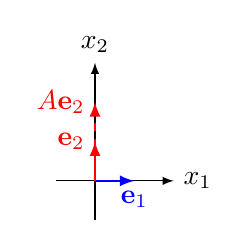
\begin{tikzpicture}[scale=0.5]
		\draw[->] (-1,0) -- (2,0) node[right] {$x_1$};
		\draw[->] (0,-1) -- (0,3) node[above] {$x_2$};
		\draw[thick, blue, ->] (0,0) -- (1,0) node[below] {$\mathbf{e}_1$};
		\draw[thick, red, ->] (0,0) -- (0,1) node[left] {$\mathbf{e}_2$};
		\draw[thick, red, dashed, ->] (0,0) -- (0,2) node[left] {$A\mathbf{e}_2$};
	\end{tikzpicture}
}

\ex{
	\(A = \begin{pmatrix} -1 & 0 \\[6pt] 0 & 1 \end{pmatrix}\)
}{
	\textbf{Transformation:} Reflection about the vertical axis.
	\centering
	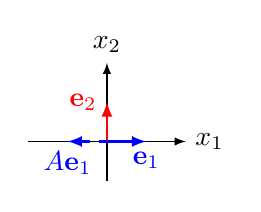
\begin{tikzpicture}[scale=0.5]
		\draw[->] (-2,0) -- (2,0) node[right] {$x_1$};
		\draw[->] (0,-1) -- (0,2) node[above] {$x_2$};
		\draw[thick, blue, ->] (0,0) -- (1,0) node[below] {$\mathbf{e}_1$};
		\draw[thick, red, ->] (0,0) -- (0,1) node[left] {$\mathbf{e}_2$};
		\draw[thick, blue, dashed, ->] (0,0) -- (-1,0) node[below] {$A\mathbf{e}_1$};
	\end{tikzpicture}
}

\ex{
	\(A = \begin{pmatrix} 0 & 1 \\[6pt] 1 & 0 \end{pmatrix}\)
}{
	\textbf{Transformation:} Reflection about the line \(x_1 = x_2\).
	\centering
	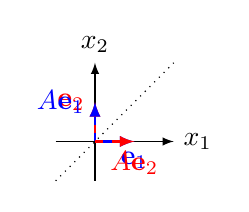
\begin{tikzpicture}[scale=0.5]
		\draw[->] (-1,0) -- (2,0) node[right] {$x_1$};
		\draw[->] (0,-1) -- (0,2) node[above] {$x_2$};
		\draw[thick, blue, ->] (0,0) -- (1,0) node[below] {$\mathbf{e}_1$};
		\draw[thick, red, ->] (0,0) -- (0,1) node[left] {$\mathbf{e}_2$};
		\draw[thick, blue, dashed, ->] (0,0) -- (0,1) node[left] {$A\mathbf{e}_1$};
		\draw[thick, red, dashed, ->] (0,0) -- (1,0) node[below] {$A\mathbf{e}_2$};
		\draw[dotted] (-1,-1) -- (2,2);
	\end{tikzpicture}
}

\ex{
	\(A = \begin{pmatrix}
		\cos\theta & -\sin\theta \\[6pt]
		\sin\theta & \cos\theta
	\end{pmatrix}\)
}{
	\textbf{Transformation:} Counterclockwise rotation by \(\theta\) about the origin.
	\centering
	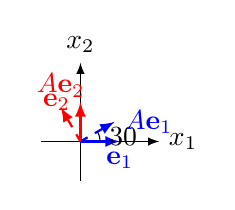
\begin{tikzpicture}[scale=0.5]
		\draw[->] (-1,0) -- (2,0) node[right] {$x_1$};
		\draw[->] (0,-1) -- (0,2) node[above] {$x_2$};
		\def\theta{30}
		\draw[thick, blue, ->] (0,0) -- (1,0) node[below] {$\mathbf{e}_1$};
		\draw[thick, red, ->] (0,0) -- (0,1) node[left] {$\mathbf{e}_2$};
		\draw[thick, blue, dashed, ->] (0,0) -- ({cos(\theta)}, {sin(\theta)}) node[right] {$A\mathbf{e}_1$};
		\draw[thick, red, dashed, ->] (0,0) -- ({-sin(\theta)}, {cos(\theta)}) node[above] {$A\mathbf{e}_2$};
		\draw (0.5,0) arc (0:\theta:0.5) node[midway, right] {$\theta$};
	\end{tikzpicture}
}

\ex{
	\(A = \begin{pmatrix} 0 & 0 \\[6pt] 0 & 1 \end{pmatrix}\)
}{
	\textbf{Transformation:} Projection onto the vertical axis.
	\centering
	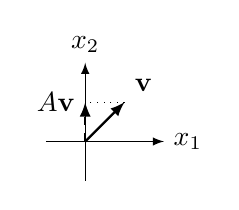
\begin{tikzpicture}[scale=0.5]
		\draw[->] (-1,0) -- (2,0) node[right] {$x_1$};
		\draw[->] (0,-1) -- (0,2) node[above] {$x_2$};
		\draw[thick, ->] (0,0) -- (1,1) node[above right] {$\mathbf{v}$};
		\draw[thick, dashed, ->] (0,0) -- (0,1) node[left] {$A\mathbf{v}$};
		\draw[dotted] (1,1) -- (0,1);
	\end{tikzpicture}
}

\section{Mapping}

\[
	[x_1,\; x_2] \;\longmapsto\; \text{point }(x_1, x_2).
\]

Under the linear transformation given by
\[
	[x_1,\; x_2] \;\mapsto\;
	\begin{bmatrix}
		x_1 + 2x_2 \\
		x_2
	\end{bmatrix},
\]
we see that points are ``stretched to the right'' in the \(x_1\)-direction, while the \(x_2\) coordinate remains unchanged.

\subsection{Method 1 -- Vector Method}

The matrix under consideration is
\[
	A \;=\; \begin{bmatrix} 1 & 2 \\ 0 & 1 \end{bmatrix}.
\]
The columns of this matrix are:
\[
	\begin{bmatrix} 1 \\ 0 \end{bmatrix}
	\quad\text{and}\quad
	\begin{bmatrix} 2 \\ 1 \end{bmatrix}.
\]
These are the images of the standard basis vectors \(\mathbf{e}_1\) and \(\mathbf{e}_2\), respectively.

\begin{center}
	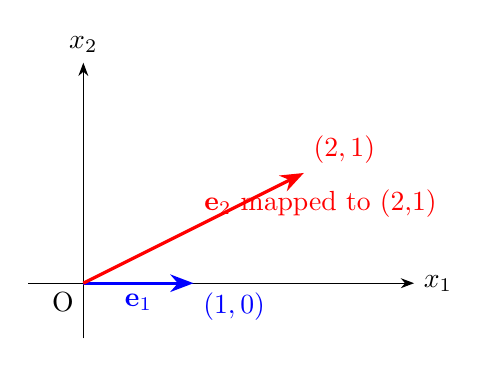
\begin{tikzpicture}[scale=1.4, >=Stealth, baseline={(0,0)}]
		% Axes
		\draw[->] (-0.5,0) -- (3,0) node[right] {\(x_1\)};
		\draw[->] (0,-0.5) -- (0,2) node[above] {\(x_2\)};

		% e1 vector
		\draw[->, very thick, blue] (0,0) -- (1,0) node[midway, below] {\(\mathbf{e}_1\)};

		% e2 vector
		\draw[->, very thick, red] (0,0) -- (2,1) node[midway, above right] {\(\mathbf{e}_2\) mapped to (2,1)};

		% Labels
		\node at (1,0) [below right, blue] {$(1,0)$};
		\node at (2,1) [above right, red] {$(2,1)$};

		\draw (0,0) node[below left] {O};
	\end{tikzpicture}
\end{center}

\subsection{Method 2 -- Vertex Method}

Consider the unit square with vertices
\[
	(0,0), \quad (1,0), \quad (1,1), \quad (0,1).
\]
We apply \(A\) to each vertex:

\[
	A \begin{bmatrix} 0 \\ 0 \end{bmatrix}
	= \begin{bmatrix} 0 \\ 0 \end{bmatrix},\quad
	A \begin{bmatrix} 1 \\ 0 \end{bmatrix}
	= \begin{bmatrix} 1 \\ 0 \end{bmatrix},\quad
	A \begin{bmatrix} 0 \\ 1 \end{bmatrix}
	= \begin{bmatrix} 2 \\ 1 \end{bmatrix},\quad
	A \begin{bmatrix} 1 \\ 1 \end{bmatrix}
	= \begin{bmatrix} 3 \\ 1 \end{bmatrix}.
\]

Hence the new vertices are \((0,0)\), \((1,0)\), \((2,1)\), and \((3,1)\). Plotting these points yields the transformed parallelogram (the image of the original unit square).

\begin{center}
	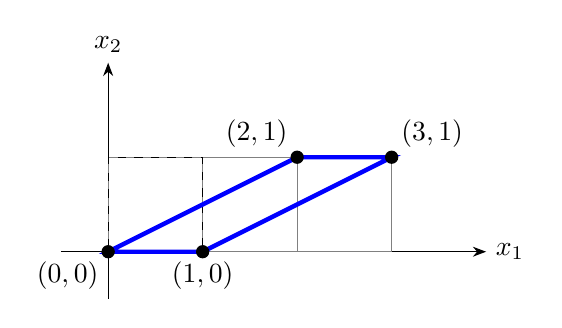
\begin{tikzpicture}[scale=1.2, >=Stealth, baseline={(0,0)}]
		% Axes
		\draw[->] (-0.5,0) -- (4,0) node[right] {\(x_1\)};
		\draw[->] (0,-0.5) -- (0,2) node[above] {\(x_2\)};

		% Original square
		\draw[very thin, gray] (0,0) grid (3,1);

		% Original square edges (dashed)
		\draw[dashed] (0,0) -- (1,0) -- (1,1) -- (0,1) -- cycle;

		% Transformed parallelogram
		\draw[ultra thick, blue] (0,0) -- (1,0) -- (3,1) -- (2,1) -- cycle;

		% Points (labels)
		\fill (0,0) circle (2pt) node[below left] {$(0,0)$};
		\fill (1,0) circle (2pt) node[below] {$(1,0)$};
		\fill (2,1) circle (2pt) node[above left] {$(2,1)$};
		\fill (3,1) circle (2pt) node[above right] {$(3,1)$};
	\end{tikzpicture}
\end{center}

\dfn{Rules for Linear Transformations}{

	\begin{enumerate}
		\item \textbf{Straight lines remain straight.}
		\item \textbf{Parallel lines remain parallel.}
		\item \textbf{Distances along lines scale in a consistent, proportional way.}
	\end{enumerate}
}

\subsubsection{Justification}

\paragraph{1. Straight lines stay straight.}
A line in parametric form is:
\[
	r(t) = t\,\mathbf{v} + \mathbf{w}.
\]
Applying \(A\) gives:
\[
	A(r(t)) = A(t\,\mathbf{v} + \mathbf{w}) = t\,A(\mathbf{v}) + A(\mathbf{w}),
\]
which is again a parametric line.

\paragraph{2. Parallel lines stay parallel.}
If two lines are parallel, their direction vectors are scalar multiples of each other. After applying \(A\), the resulting direction vectors are \(A(\mathbf{v})\) for each original direction \(\mathbf{v}\). Since \(A\) is linear, any scalar multiples remain so, preserving parallelism.

\paragraph{3. Distances scale proportionally.}
For two points \(\mathbf{v}_1\) and \(\mathbf{v}_2\), the difference is \(\mathbf{d} = \mathbf{v}_2 - \mathbf{v}_1\). Under \(A\):
\[
	A\mathbf{v}_2 - A\mathbf{v}_1 = A(\mathbf{v}_2 - \mathbf{v}_1) = A(\mathbf{d}).
\]
Thus the new distance \(\|\mathbf{d}'\| = \|A(\mathbf{d})\|\) is a consistent transform of \(\|\mathbf{d}\|\), depending on the nature of \(A\).

\ex{
	A matrix \(A\) that acts on a parallelogram (spanned by two vectors \(\mathbf{x}_1, \mathbf{x}_2\)) will produce another parallelogram in the output plane.
}{
	\begin{center}
		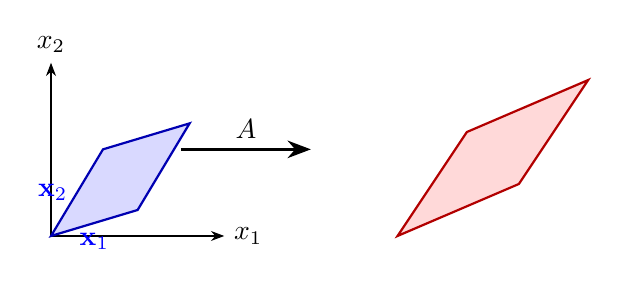
\begin{tikzpicture}[scale=1.1, >=Stealth, baseline={(0,0)}]
			% Original parallelogram
			\coordinate (O) at (0,0);
			\coordinate (X1) at (1,0.3);
			\coordinate (X2) at (0.6,1);

			\draw[->] (O) -- ++(2,0) node[right] {\(x_1\)};
			\draw[->] (O) -- ++(0,2) node[above] {\(x_2\)};

			\filldraw[fill=blue!15, draw=blue!70!black, thick]
			(O) -- (X1) -- ($(X1)+(X2)$) -- (X2) -- cycle;
			\node at ($(X1)!0.5!(O)$) [below, blue] {\(\mathbf{x}_1\)};
			\node at ($(X2)!0.5!(O)$) [left, blue] {\(\mathbf{x}_2\)};

			% Arrow indicating transformation
			\draw[->, very thick] (1.5,1) -- (3,1) node[midway, above] {$A$};

			% Transformed parallelogram
			% Let's define some coordinates for the transformed shape
			\coordinate (O2) at (4,0);               % Shift for the second shape
			\coordinate (X1t) at ($(O2)+(1.4,0.6)$); % Some transformed version of x1
			\coordinate (X2t) at ($(O2)+(0.8,1.2)$); % Some transformed version of x2

			\filldraw[fill=red!15, draw=red!70!black, thick]
			(O2) -- (X1t) -- ($(X1t)+(X2t)-(O2)$) -- (X2t) -- cycle;
		\end{tikzpicture}
	\end{center}

	\noindent
	\emph{Here, lines remain lines, parallels remain parallel.}
}

\section{A System of Linear Equations}

We have a matrix \(A\) of size \(m \times n\), multiplying an unknown vector
\(\begin{bmatrix} x_1 \\ x_2 \\ \vdots \\ x_n \end{bmatrix}\)
(which belongs to \(\mathbb{R}^n\)), producing a result vector
\(\begin{bmatrix} v_1 \\ v_2 \\ \vdots \\ v_m \end{bmatrix}\)
in \(\mathbb{R}^m\):
\[
	A_{m \times n}
	\begin{bmatrix}
		x_1    \\
		x_2    \\
		\vdots \\
		x_n
	\end{bmatrix}
	=
	\begin{bmatrix}
		v_1    \\
		v_2    \\
		\vdots \\
		v_m
	\end{bmatrix}.
\]

This can be viewed as a \emph{system of \(m\) linear equations in \(n\) unknowns}. We are often interested in two main questions:

\begin{enumerate}
	\item \textbf{Does a solution exist?}
	      That is, can we find \(x_1, x_2, \dots, x_n\) so that \(A\mathbf{x} = \mathbf{v}\)?
	      Geometrically, this asks if \(\mathbf{v}\) lies in the \emph{column space} (or image) of \(A\).

	\item \textbf{If at least one solution exists, is it unique or are there infinitely many?}
	      Uniqueness is typically tied to whether the columns of \(A\) are linearly independent (and whether \(m\), \(n\) are related in a way that gives a single solution).  If there are \emph{fewer} pivots than unknowns, or if the system is underdetermined, infinitely many solutions can occur.
\end{enumerate}

\vspace{1em}
\noindent
\textit{Key intuition:}
\begin{itemize}
	\item The question of \emph{existence} boils down to whether \(\mathbf{v}\) is in the span of the columns of \(A\).
	\item The question of \emph{uniqueness} depends on whether those columns form a set of independent vectors and on the relationship between \(m\) and \(n\).
\end{itemize}


\section{How to Determine Consistency, Uniqueness, and the Number of Solutions for a Linear System}
\nt{
	We consider a linear system
	\[
		\begin{cases}
			a_{11} x_1 \;+\; a_{12} x_2 \;+\; \cdots + a_{1n} x_n \;=\; b_1 \\[6pt]
			a_{21} x_1 \;+\; a_{22} x_2 \;+\; \cdots + a_{2n} x_n \;=\; b_2 \\
			\vdots &                                                        \\
			a_{m1} x_1 \;+\; a_{m2} x_2 \;+\; \cdots + a_{mn} x_n \;=\; b_m
		\end{cases}
	\]
	and write it in \emph{augmented matrix} form:
	\[
		\bigl[A \mid \mathbf{b}\bigr]
		\;=\;
		\begin{bmatrix}
			a_{11} & a_{12} & \cdots & a_{1n} & b_1    \\
			a_{21} & a_{22} & \cdots & a_{2n} & b_2    \\
			\vdots & \vdots & \ddots & \vdots & \vdots \\
			a_{m1} & a_{m2} & \cdots & a_{mn} & b_m
		\end{bmatrix}.
	\]

	\begin{itemize}
		\item We perform \emph{elementary row operations} (EROs) on \(\bigl[A \mid \mathbf{b}\bigr]\) to attempt to solve the system. The EROs are:
		      \begin{enumerate}
			      \item \textbf{Scaling (multiplying a row by a nonzero constant).}
			      \item \textbf{Row replacement} (\(R_i \;=\; R_i \;+\; c\,R_j\) for \(i\neq j\)).
			      \item \textbf{Interchanging two rows} (\(R_i \leftrightarrow R_j\)).
		      \end{enumerate}
		      These operations do not change the solution set of the system.
	\end{itemize}

	\textbf{Row Echelon Form (REF)}
	We say \(\bigl[A\mid\mathbf{b}\bigr]\) is in \emph{row echelon form} if:
	\begin{itemize}
		\item All rows of all zeros (if any) are at the bottom of the matrix.
		\item Each \emph{pivot} (leftmost nonzero entry in a nonzero row) is strictly to the right of the pivot in the row above.
	\end{itemize}
	A pivot column in \(A\) corresponds to a \emph{leading variable} (or \emph{basic variable}), and any other column (apart from the augmented column) is called a \emph{free column} (its corresponding variable is a \emph{free variable}).

	\textbf{Consistency \& Number of Solutions}
	\begin{itemize}
		\item If, in the augmented matrix, there is a pivot in the last column (meaning a row of the form
		      \[
			      [\,0\quad 0\quad \cdots\quad 0 \mid c\,],\quad c \neq 0,
		      \]
		      ) then the system is \emph{inconsistent} (no solutions). This corresponds to an equation \(0 = c\) where \(c\neq 0\), which is impossible.
		\item If no such contradiction is found, then at least one solution exists (the system is \emph{consistent}).
		\item The number of pivot columns in \(A\) (i.e.\ the number of leading variables) tells us whether solutions are unique or infinite:
		      \begin{enumerate}
			      \item If the number of pivots equals the number of unknowns \(n\), then there is exactly one solution (assuming no inconsistency).
			      \item If the number of pivots is less than \(n\), then there are free variables, implying infinitely many solutions (again, assuming no inconsistency).
		      \end{enumerate}
	\end{itemize}

	\ex{Example: Augmented Matrix and REF}{
		\[
			\begin{bmatrix}
				1 & 2 & 3 & 5  \\
				2 & 4 & 6 & 9  \\
				3 & 6 & 9 & 15
			\end{bmatrix}
			\;\longrightarrow\;\text{(REF)}.
		\]
		One performs row operations to get an upper-triangular or echelon form.  If the last row becomes something like
		\[
			[\,0\;\;0\;\;0\mid c\,], \quad c\neq 0,
		\]
		then there is no solution.  Otherwise, we identify pivot columns, read off the relationships among variables, and find a general solution (unique or infinite).
	}

	\dfn{Free Columns and Basic Columns}{
		Once an augmented matrix is in REF, we label each pivot column (in \(A\)) as a \emph{basic column}, and any other column (except the last augmented column) as a \emph{free column}.
		\begin{itemize}
			\item If \(x_j\) corresponds to a free column, we may label \(x_j\) as a parameter (e.g.\ \(t_1, t_2, \dots\)).
			\item The variables in pivot columns can then be written in terms of these parameters.
		\end{itemize}
		In this manner, we get a general solution describing the entire solution set to \(A\mathbf{x} = \mathbf{b}\).
	}

	\textbf{Algorithm to Convert \(\bigl[A\mid \mathbf{b}\bigr]\) to \(\mathrm{REF}(A)\)}
	\begin{enumerate}
		\item \emph{Select a candidate row}: Choose the topmost row \emph{among those not yet having a pivot} in which a pivot might appear.
		\item \emph{Pivot search and possible row swap}: Among this candidate row and those below it, find a row having a leftmost nonzero entry in the desired pivot column. Interchange (swap) that row with the candidate row if needed, placing a nonzero entry where your pivot should be.
		\item \emph{Declare the pivot and eliminate below}: Scale the pivot row (if desired) so that the pivot becomes \(1\). Then use row replacement to produce zeros below that pivot in the same column.
		\item Move to the next row down and next column to the right, and repeat until you have a row echelon form.
	\end{enumerate}

	One can then further use row replacement operations to clear the entries \emph{above} each pivot, yielding the \emph{reduced} row echelon form (RREF). However, for most solution purposes, REF is already sufficient to read off whether solutions exist, how many, and so on.
}
\subsection{FRR}
\begin{algorithm}[H]
	\KwIn{Matrix \(A\) of size \(m \times n\) and vector \(\mathbf{b}\) of size \(m\)}
	\KwOut{Upper triangular matrix \(A\) and modified vector \(\mathbf{b}\)}
	\SetAlgoLined
	\SetNoFillComment
	\tcc{Forward elimination process}
	\For{$k \leftarrow 1$ \KwTo $\min(m, n)$}{
		\For{$i \leftarrow k+1$ \KwTo $m$}{
			\If{$A_{kk} \neq 0$}{
				$f \leftarrow A_{ik} / A_{kk}$\;
				\For{$j \leftarrow k$ \KwTo $n$}{
					$A_{ij} \leftarrow A_{ij} - f \cdot A_{kj}$\;
				}
				$b_i \leftarrow b_i - f \cdot b_k$\;
			}
		}
	}
	\Return $A, \mathbf{b}$\;
	\caption{Forward Row Reduction (Forward Elimination)}
\end{algorithm}

\section{Back Row Reduction}

\nt{
	Back row reduction, also known as back substitution, is a method used to solve a system of linear equations that has been transformed into an upper triangular form through Gaussian elimination. This method involves solving the equations starting from the last row and moving upwards.
}

\dfn{Back Row Reduction}{
	Consider a system of linear equations represented in matrix form as \(A\mathbf{x} = \mathbf{b}\), where \(A\) is an upper triangular matrix:
	\[
		\begin{bmatrix}
			a_{11} & a_{12} & \cdots & a_{1n} \\
			0      & a_{22} & \cdots & a_{2n} \\
			\vdots & \vdots & \ddots & \vdots \\
			0      & 0      & \cdots & a_{nn}
		\end{bmatrix}
		\begin{bmatrix}
			x_1    \\
			x_2    \\
			\vdots \\
			x_n
		\end{bmatrix}
		=
		\begin{bmatrix}
			b_1    \\
			b_2    \\
			\vdots \\
			b_n
		\end{bmatrix}.
	\]
	The solution is obtained by solving the last equation first and then substituting the obtained values into the preceding equations.
}

\ex{Example of Back Row Reduction}{
	Consider the following upper triangular system:
	\[
		\begin{cases}
			2x_1 + 3x_2 + 4x_3 = 5, \\
			0x_1 + 6x_2 + 7x_3 = 8, \\
			0x_1 + 0x_2 + 9x_3 = 10.
		\end{cases}
	\]
	We start with the last equation:
	\[
		9x_3 = 10 \quad \Rightarrow \quad x_3 = \frac{10}{9}.
	\]
	Next, we substitute \(x_3\) into the second equation:
	\[
		6x_2 + 7\left(\frac{10}{9}\right) = 8 \quad \Rightarrow \quad 6x_2 + \frac{70}{9} = 8 \quad \Rightarrow \quad 6x_2 = 8 - \frac{70}{9} \quad \Rightarrow \quad x_2 = \frac{2}{9}.
	\]
	Finally, we substitute \(x_2\) and \(x_3\) into the first equation:
	\[
		2x_1 + 3\left(\frac{2}{9}\right) + 4\left(\frac{10}{9}\right) = 5 \quad \Rightarrow \quad 2x_1 + \frac{6}{9} + \frac{40}{9} = 5 \quad \Rightarrow \quad 2x_1 = 5 - \frac{46}{9} \quad \Rightarrow \quad x_1 = \frac{1}{9}.
	\]
	Thus, the solution is:
	\[
		x_1 = \frac{1}{9}, \quad x_2 = \frac{2}{9}, \quad x_3 = \frac{10}{9}.
	\]
}

\begin{algorithm}[H]
	\KwIn{Upper triangular matrix \(A\) of size \(n \times n\) and vector \(\mathbf{b}\) of size \(n\)}
	\KwOut{Solution vector \(\mathbf{x}\) of size \(n\)}
	\SetAlgoLined
	\SetNoFillComment
	\tcc{Initialize solution vector}
	\For{$i \leftarrow n$ \KwTo $1$}{
		$x_i \leftarrow b_i$\;
		\For{$j \leftarrow i+1$ \KwTo $n$}{
			$x_i \leftarrow x_i - A_{ij} \cdot x_j$\;
		}
		$x_i \leftarrow x_i / A_{ii}$\;
	}
	\Return $\mathbf{x}$\;
	\caption{Back Row Reduction (Back Substitution)}
\end{algorithm}

\ex{Full SLE solving}{
	$$ \begin{bmatrix}
			1 & 1  & 2 & 2  \\
			1 & -1 & 0 & -2 \\
			2 & 0  & m & 0
		\end{bmatrix}
	$$
	$$
		\begin{bmatrix}
			1 & 1  & 2   & 2  \\
			0 & -2 & -2  & -4 \\
			0 & -2 & m-4 & -4
		\end{bmatrix}
	$$
	$$
		\begin{bmatrix}
			1 & 1  & 2   & 2  \\
			0 & -2 & -2  & -4 \\
			0 & 0  & m-2 & 0
		\end{bmatrix}
	$$
	given m=0
	$$
		\begin{bmatrix}
			1 & 1  & 2  & 2  \\
			0 & -2 & -2 & -4 \\
			0 & 0  & 0  & 0
		\end{bmatrix}
	$$
	$$
		\begin{bmatrix}
			1 & 1 & 2 & 2 \\
			0 & 1 & 1 & 2 \\
			0 & 0 & 0 & 0
		\end{bmatrix}
	$$
	$$
		\begin{bmatrix}
			1 & 0 & 1 & 0 \\
			0 & 1 & 1 & 2 \\
			0 & 0 & 0 & 0
		\end{bmatrix}
	$$

}

\chapter{Linear Combinations}



\section{Matrix--Vector Product as Linear Combination}

\[
	\begin{aligned}
		A x
		 & =
		\begin{bmatrix}
			1 & -2  \\[6pt]
			3 & \;2
		\end{bmatrix}
		\begin{bmatrix}
			x_1 \\[3pt]
			x_2
		\end{bmatrix}
		= x_1
		\begin{bmatrix} 1 \\[3pt] 3 \end{bmatrix}
		+ x_2
		\begin{bmatrix} -2 \\[3pt] 2 \end{bmatrix}
		= b.
	\end{aligned}
\]

\textit{Intuition:} ``Scaling each column of \(A\) by its corresponding entry in \(x\).''

In other words, to compute \(A x\), you take \(x_1\) times the first column of \(A\) plus \(x_2\) times the second column of \(A\).


\ex{ A Specific Choice of \(x\)}{
	If
	\[
		A =
		\begin{bmatrix}
			1 & -2    \\[3pt]
			3 & \;\,2
		\end{bmatrix},
	\]
	then the first column is
	\[
		a_1 = \begin{bmatrix} 1 \\ 3 \end{bmatrix}
		\quad\text{and}\quad
		a_2 = \begin{bmatrix} -2 \\ 2 \end{bmatrix}.
	\]
	A linear combination of these columns is
	\[
		x_1 \begin{bmatrix} 1 \\ 3 \end{bmatrix}
		\;+\;
		x_2 \begin{bmatrix} -2 \\ 2 \end{bmatrix}
		\;=\;
		b.
	\]

	As an example, if \(x_1 = -\tfrac{1}{3}\) and \(x_2 = 1\),
	\[
		-\tfrac{1}{3}
		\begin{bmatrix} 1 \\ 3 \end{bmatrix}
		\;+\;
		\begin{bmatrix} -2 \\ 2 \end{bmatrix}
		=
		\begin{bmatrix}
			-\tfrac{1}{3} - 2 \\[4pt]
			-1 + 2
		\end{bmatrix}
		=
		\begin{bmatrix}
			-\tfrac{7}{3} \\[4pt]
			1
		\end{bmatrix}.
	\]
	In the notes, a similar combination yields \(\begin{bmatrix}-2 \\ -2\end{bmatrix}\). The key point is that any pair \((x_1,x_2)\) gives a vector in \(\mathbb{R}^2\).
}

\dfn{Span}{
	\textbf{Span} of a set of vectors is the collection of all linear combinations of those vectors. Concretely, for
	\[
		a_1 = \begin{bmatrix} 1 \\ 3 \end{bmatrix},
		\quad
		a_2 = \begin{bmatrix} -2 \\ 2 \end{bmatrix},
	\]
	we write
	\[
		\mathrm{Span}\{\,a_1, a_2\}
		=\Bigl\{\,
		x_1 a_1 + x_2 a_2
		\;\big|\;
		x_1, x_2 \in \mathbb{R}
		\Bigr\}.
	\]
	Any vector \(b\) not in this span means \(A x = b\) has no solution.
}

\section{Linear Combinations and the Span}
Vectors ``outside'' the span of \(\{a_1,a_2\}\) are precisely those \(b\) for which the system \(A x = b\) is not consistent. Equivalently, they are not expressible as a linear combination of \(a_1\) and \(a_2\).


\section{Geometric Plots in the Notes}

\begin{enumerate}
	\item \textit{First Plot (showing the columns \(a_1\) and \(a_2\)):}

	      \begin{center}
		      \begin{tikzpicture}[scale=0.8,>=stealth]
			      % axes
			      \draw[->] (-0.5,0) -- (3.5,0) node[right] {\(x\)};
			      \draw[->] (0,-0.5) -- (0,3.5) node[above] {\(y\)};

			      % a_1 vector
			      \draw[->,thick,blue] (0,0) -- (1,3) node[midway,left] {\(\displaystyle a_1\)};

			      % a_2 vector
			      \draw[->,thick,red] (0,0) -- (-2,2) node[midway,above] {\(\displaystyle a_2\)};

			      % a rough parallelogram to illustrate a typical combination
			      \draw[dashed] (1,3) -- (1-2,3+2);
			      \draw[dashed] (-2,2) -- (-2+1,2+3);
		      \end{tikzpicture}
	      \end{center}

	      Any linear combination \(x_1 a_1 + x_2 a_2\) lands in the parallelogram structure (and its extensions) formed by these two vectors.

	\item \textit{Second Plot (showing a vector not in the span)}:

	      \begin{center}
		      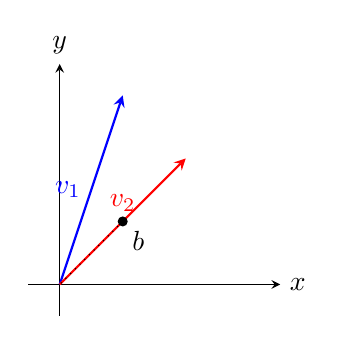
\begin{tikzpicture}[scale=0.8,>=stealth]
			      % axes
			      \draw[->] (-0.5,0) -- (3.5,0) node[right] {\(x\)};
			      \draw[->] (0,-0.5) -- (0,3.5) node[above] {\(y\)};

			      % example vectors v1, v2 (suppose they are the same as above or placeholders)
			      \draw[->,thick,blue] (0,0) -- (1,3) node[midway,left] {\(\displaystyle v_1\)};
			      \draw[->,thick,red] (0,0) -- (2,2) node[midway,above] {\(\displaystyle v_2\)};

			      % a point b that is not in the span
			      \filldraw[black] (1,1) circle (2pt) node[below right] {\(\displaystyle b\)};

			      % dashed lines to illustrate that b is not on the plane spanned by v1 and v2
			      % (just a conceptual marker)
			      \draw[dotted] (1,1) -- (0,0);
		      \end{tikzpicture}
	      \end{center}

	      If \(v_1\) and \(v_2\) do not cover \((1,1)\) by any linear combination, then \(\begin{bmatrix}1\\1\end{bmatrix}\) is not in their span, hence no solution exists for \(Ax=b\).

	\item \textit{Plot illustrating parallel vectors}:

	      \begin{center}
		      \begin{tikzpicture}[scale=0.8,>=stealth]
			      % axes
			      \draw[->] (-0.5,0) -- (4,0) node[right] {\(x\)};
			      \draw[->] (0,-0.5) -- (0,4) node[above] {\(y\)};

			      % two parallel vectors
			      \draw[->,thick,blue] (0,0) -- (2,2) node[midway,above left] {\(\displaystyle v_1\)};
			      \draw[->,thick,blue!50!green] (0,0) -- (3,3) node[midway,above] {\(\displaystyle v_2\)};

			      % a vector b not on that line
			      \filldraw[red] (2,3) circle (2pt) node[right] {\(\displaystyle b\)};

			      % line indication
			      \draw[dashed] (0,0) -- (3.5,3.5);
		      \end{tikzpicture}
	      \end{center}

	      Here, \(v_1\) and \(v_2\) are multiples of each other, so their span is just the single dashed line. The vector \(b\) off that line cannot be written as any combination of \(v_1\) and \(v_2\).
\end{enumerate}

\ex{$\vec{b}$ not in span of $\vec{v_1}, \vec{v_2}$}{
	\tdplotsetmaincoords{70}{110}
	\centering
	\begin{tikzpicture}[tdplot_main_coords, scale=2]
		% Draw coordinate axes
		\draw[->, thick] (0,0,0) -- (2,0,0) node[anchor=north east] {$x$};
		\draw[->, thick] (0,0,0) -- (0,2,0) node[anchor=north west] {$y$};
		\draw[->, thick] (0,0,0) -- (0,0,2) node[anchor=south] {$z$};

		% Draw the plane spanned by v1 and v2.
		% Every vector in the span has x = y, so we fill the plane { (u,u,w) : u,w in R }.
		% Here we choose a rectangular patch with u from -1 to 1 and w from -1 to 2.
		\filldraw[fill=blue!20, draw=blue, opacity=0.5]
		(-1,-1,-1) -- (1,1,-1) -- (1,1,2) -- (-1,-1,2) -- cycle;

		% Draw vector v1 = (1,1,1)
		\draw[-{Stealth[scale=1.2]}, red, thick] (0,0,0) -- (1,1,1)
		node[midway, anchor=south east] {$v_1$};

		% Draw vector v2 = (-1,-1,1)
		\draw[-{Stealth[scale=1.2]}, red, thick] (0,0,0) -- (-1,-1,1)
		node[midway, anchor=north west] {$v_2$};

		% Draw vector b = (1,0,0)
		\draw[-{Stealth[scale=1.2]}, green!70!black, thick] (0,0,0) -- (1,0,0)
		node[midway, anchor=south] {$b$};

		% Add an annotation that b is not in the span of v1 and v2.
		\node at (2.5, 2, 0.5) {$b\notin\operatorname{span}\{v_1,v_2\}$};
	\end{tikzpicture}
}

\subsection{Key Conclusions}

\begin{itemize}
	\item \(\mathrm{Span}\{a_1, a_2\}\) is the set of all vectors \(b\) for which \(Ax = b\) has a solution.
	\item If \(b\) is not in that span, there is no solution.
	\item Geometrically, if \(a_1\) and \(a_2\) are not multiples of each other, their span is a 2D plane through the origin in \(\mathbb{R}^2\). If they are multiples, the span is just a single line, and most vectors in \(\mathbb{R}^2\) lie outside that line (no solution).
	\item $span{a_1}$ is a line or point. $span{a_1, a_2}$ is a plane, line or point. and so on
\end{itemize}

\subsection{Dropping a vector to retain the same span}

\qs{Drop vector $a_3$ to retain the same span as $a_1$, $a_2$ and $a_3$.}{
	\[
		a_1 =
		\begin{bmatrix}
			2 \\ 1
		\end{bmatrix}
	\]

	\[
		a_2 =
		\begin{bmatrix}
			1 \\ 1
		\end{bmatrix}
	\]

	\[
		a_3 =
		\begin{bmatrix}
			3 \\ 3
		\end{bmatrix}
	\]
}

\sol
yes, $span{a_1,a_2,a_3}=span{a_1,a_2}$ because $a_3$ is a linear combination of $a_1$ and $a_2$ ($a_1+a_2a_3$)

\section{Evaluating Linear Dependence Procedurally}

\ex{
	Finding linear dependence of a set of vectors.
}{
	\[
		\vec{v_1} =
		\begin{bmatrix}
			1 \\2\\3
		\end{bmatrix}
		,
		\vec{v_2} =
		\begin{bmatrix}
			3 \\2\\1
		\end{bmatrix}
		,
		\vec{v_3} =
		\begin{bmatrix}
			5 \\2\\-1
		\end{bmatrix}
	\]
	Since $v_3$ is a linear combination of $v_1$ and $v_2$, we can drop $v_3$ to retain the same span as $v_1$ and $v_2$.
	\[
		span{v_1,v_2,v_3} = span{v_1,v_2}
	\]
	As
	\[
		v_3 = 2v_1 - v_2
	\]
}

\nt{Working towards a procedure for evaluating linear dependence of a set of vectors.}

\[
	-v_1 + 2v_2 -v_3 = 0
\]

\[
	\begin{bmatrix}
		\vec{v_1} & \vec{v_2} & \vec{v_3}
	\end{bmatrix}
	\begin{bmatrix}
		x_1 \\ x_2 \\ x_3
	\end{bmatrix}
	=
	\begin{bmatrix}
		0 \\ 0 \\ 0
	\end{bmatrix}
\]

We know that one solution is

\[
	\begin{bmatrix}
		x_1 \\ x_2 \\ x_3
	\end{bmatrix}
	=
	\begin{bmatrix}
		-1 \\2\\-1
	\end{bmatrix}
\]

Since this SLE has one particular solution as well as the trivial one, then it must have infinitely many solutions.\\
Then if \(A \vec{x} = 0\) has infinitely many solutions, then the set of vectors (columns) in \(A\) is linearly dependent.\\
Conversely, if \(A \vec{x} = 0\) has only one solution $(\vec{x} = \vec{0})$, then the set of vectors (columns) in \(A\) is linearly independent.\\

\dfn{Linear Independence}{
	We say a set of vectors $\{v_1, v_2, \cdots, v_n\}$ is \emph{linearly independent} if the only solution to the SLE
	\[
		\begin{bmatrix}
			\vec{v_1} & \vec{v_2} & \cdots & \vec{v_n}
		\end{bmatrix}
		\begin{bmatrix}
			x_1 \\ x_2 \\ \vdots \\ x_n
		\end{bmatrix}
		=
		\begin{bmatrix}
			0 \\ 0 \\ \vdots \\ 0
		\end{bmatrix}
	\]
	is the trivial solution, i.e. $\vec{x} = \vec{0}$.\\
}

\[
	A' =
	\begin{bmatrix}
		1 & 3 & 5  & 0 \\
		2 & 2 & 2  & 0 \\
		3 & 1 & -1 & 0
	\end{bmatrix}
	\xrightarrow{R_2 = R_2 - 2R_1, \quad R_3 = R_3 - 3R_1}
	\begin{bmatrix}
		1 & 3  & 5   & 0 \\
		0 & -4 & -8  & 0 \\
		0 & -8 & -16 & 0
	\end{bmatrix}
	\xrightarrow{R_3 = R_3 - 2R_2}
	\begin{bmatrix}
		1 & 3  & 5  & 0 \\
		0 & -4 & -8 & 0 \\
		0 & 0  & 0  & 0
	\end{bmatrix}
	= \text{REF}(A')
\]

1 Free variable $\implies$ Linearly Independent

\[
	\text{REF}(A')
	\xrightarrow{R_2 = R_2 / (-4)}
	\begin{bmatrix}
		1 & 3 & 5 & 0 \\
		0 & 1 & 2 & 0 \\
		0 & 0 & 0 & 0
	\end{bmatrix}
	\xrightarrow{R_1 = R_1 - 3R_2}
	\begin{bmatrix}
		1 & 0 & -1 & 0 \\
		0 & 1 & 2  & 0 \\
		0 & 0 & 0  & 0
	\end{bmatrix}
	= \text{RREF}(A')
	\begin{bmatrix}
		x_1 \\
		x_2 \\
		x_3
	\end{bmatrix}
\]

Then

\[
	\begin{bmatrix}
		\vec{v_1} & \vec{v_2} & \vec{v_3}
	\end{bmatrix}
	t_3
	\begin{bmatrix}
		1 \\-2\\1
	\end{bmatrix}
	=
	\begin{bmatrix}
		0 \\0\\0
	\end{bmatrix}
\]

And therefore the linear combination in its homogeneous form implies

\[
	t_3 (\vec{v_1} - 2\vec{v_2} + \vec{v_3}) = \vec{0}
\]

\section{Identity Matrix}

\dfn{Identity Matrix}{
	special Square matrix where the diagonal elements are 1 and the off-diagonal elements are 0.

	\[
		I_n =
		\begin{bmatrix}
			1      & 0      & \cdots & 0      \\
			0      & 1      & \cdots & 0      \\
			\vdots & \vdots & \ddots & \vdots \\
			0      & 0      & \cdots & 1
		\end{bmatrix}
	\]
	Note that
	\(I_n \vec{x} = \vec{x}\)
	and
	\(I_n' = I_n\)
	and therefore is called a \textbf{symmetric matrix}
}

\qs{
	Matrix Multiplication that gives Identity matrix
}{
	\[
		A=
		\begin{bmatrix}
			1 & 0.7 \\
			0 & 1
		\end{bmatrix}
	\]
	Find a matrix $B$ such that
	$$AB=I$$
}
\sol
Since \(A\) makes a horizontal shear of $0.7$ then \(B\) should do the opposite

\[
	\therefore B =
	\begin{bmatrix}
		1 & -0.7 \\
		0 & 1
	\end{bmatrix}
	= A^{-1}
\]

\qs{
	Matrix Multiplication that gives Identity matrix 2
}{
	\[
		A=
		\begin{bmatrix}
			-1 & 0 \\
			0  & 1
		\end{bmatrix}
	\]
	Find a matrix $B$ such that
	$$AB=I$$
}

\sol
Since \(A\) makes a reflection about the \(x_2\) axis, \(B\) must do the same

\[
	\therefore B =
	\begin{bmatrix}
		-1 & 0 \\
		0  & 1
	\end{bmatrix}
	= A^{-1}
\]

\qs{
	Matrix Multiplication that gives Identity matrix
}{
	\[
		A=
		\begin{bmatrix}
			1 & 0 \\
			0 & 0
		\end{bmatrix}
	\]
	Find a matrix $B$ such that
	$$AB=I$$
}

\sol
\(A\) flattens all vertical components. Geometrically speaking, \(A^{-1}\) doesn't exist, as shown here\\

\[
	\begin{bmatrix}
		1 & 0 \\
		0 & 0
	\end{bmatrix}
	\cdot
	\begin{bmatrix}
		a & b \\
		c & d
	\end{bmatrix}
	=
	\begin{bmatrix}
		a & b \\
		0 & 0
	\end{bmatrix}
\]

Observe that \(span{A}\) is the line \(x_2=0\)\\

\dfn{General Case for inverses of square matrices}{
	For a matrix \(A\) which is \(n \times n\), $A^{-1}$ exists if and only if
	$$span \{  A \} = \mathbb{R}^{n} $$
}

\dfn{Finding \(A^{-1}\)}{

Get the Augmented matrix $$A''=[\,A \,|\,I\,]$$ where \(A\,,\,I\) are in the form \(n \times n \) and then perform RREF on this augmented matrix. Once done, you will have a matrix in the form $$RREF(A'')=[\,I\,|\,A^{-1}\,]$$

}

\ex{Finding \(A^{-1}\)}{
	\[
		A=
		\begin{bmatrix}
			1 & 0.7 \\
			0 & 1
		\end{bmatrix}
	\]
	\[
		A''=
		\begin{bmatrix}
			1 & 0.7 & 1 & 0 \\
			0 & 1   & 0 & 1
		\end{bmatrix}
	\]
	Then RREF
	\[
		\xrightarrow{R_1=R_1-0.7R_2}
		\begin{bmatrix}
			1 & 0 & 1 & -0.7 \\
			0 & 1 & 0 & 1
		\end{bmatrix}
	\]
	\[
		\therefore
		A^{-1}=
		\begin{bmatrix}
			1 & -0.7 \\
			0 & 1
		\end{bmatrix}
	\]
}

\ex{Finding \(A^{-1}\)}{
\[
	A=
	\begin{bmatrix}
		1 & 3 & 2 \\
		2 & 2 & 1 \\
		3 & 1 & 3
	\end{bmatrix}
\]
Check if \(span \{ A \} = \mathbb{R}^3\)
\[
	\xrightarrow{
		\begin{aligned}
			R_2=R_2-2R_1 \\
			R_3=R_3-3R_1
		\end{aligned}
	}
	\begin{bmatrix}
		1 & 3  & 2  \\
		0 & -4 & -3 \\
		0 & -8 & -3
	\end{bmatrix}
	\xrightarrow{R_3=R_3-2R_2}
	\begin{bmatrix}
		\tikz[baseline=(char.base)] \node[draw,circle,inner sep=2pt] (char) {1}; & 3                                                                         & 2                                                                        \\
		0                                                                        & \tikz[baseline=(char.base)] \node[draw,circle,inner sep=2pt] (char) {-4}; & -3                                                                       \\
		0                                                                        & 0                                                                         & \tikz[baseline=(char.base)] \node[draw,circle,inner sep=2pt] (char) {3};
	\end{bmatrix}
\]
Here \(A\) has 3 pivots, so it is invertible. Next, make the augmented matrix \(A''=[\,A \,|\,I\,]\) and perform RREF
\[
	\begin{bmatrix}
		1 & 3 & 2 & 1 & 0 & 0 \\
		2 & 2 & 1 & 0 & 1 & 0 \\
		3 & 1 & 3 & 0 & 0 & 1
	\end{bmatrix}
\]
\[
	\begin{bmatrix}
		1 & 3 & 2 & 1 & 0 & 0 \\
		2 & 2 & 1 & 0 & 1 & 0 \\
		3 & 1 & 3 & 0 & 0 & 1
	\end{bmatrix}
	\xrightarrow{
		\begin{aligned}
			R_2 & = R_2-2R_1 \\[4pt]
			R_3 & = R_3-3R_1
		\end{aligned}
	}
	\begin{bmatrix}
		1 & 3  & 2  & 1  & 0 & 0 \\
		0 & -4 & -3 & -2 & 1 & 0 \\
		0 & -8 & -3 & -3 & 0 & 1
	\end{bmatrix}
	\xrightarrow{R_3=R_3-2R_2}
	\begin{bmatrix}
		1 & 3  & 2  & 1  & 0  & 0 \\
		0 & -4 & -3 & -2 & 1  & 0 \\
		0 & 0  & 3  & 1  & -2 & 1
	\end{bmatrix}
\]
\[
	\xrightarrow{R_2=-\frac{1}{4}R_2}
	\begin{bmatrix}
		1 & 3 & 2           & 1           & 0            & 0 \\
		0 & 1 & \frac{3}{4} & \frac{1}{2} & -\frac{1}{4} & 0 \\
		0 & 0 & 3           & 1           & -2           & 1
	\end{bmatrix}
	\xrightarrow{R_1=R_1-3R_2}
	\begin{bmatrix}
		1 & 0 & -\frac{1}{4} & -\frac{1}{2} & \frac{3}{4}  & 0 \\
		0 & 1 & \frac{3}{4}  & \frac{1}{2}  & -\frac{1}{4} & 0 \\
		0 & 0 & 3            & 1            & -2           & 1
	\end{bmatrix}
\]
\[
	\xrightarrow{R_3=\frac{1}{3}R_3}
	\begin{bmatrix}
		1 & 0 & -\frac{1}{4} & -\frac{1}{2} & \frac{3}{4}  & 0           \\
		0 & 1 & \frac{3}{4}  & \frac{1}{2}  & -\frac{1}{4} & 0           \\
		0 & 0 & 1            & \frac{1}{3}  & -\frac{2}{3} & \frac{1}{3}
	\end{bmatrix}
	\xrightarrow{
		\begin{aligned}
			R_1 & = R_1+\frac{1}{4}R_3 \\[4pt]
			R_2 & = R_2-\frac{3}{4}R_3
		\end{aligned}
	}
	\begin{bmatrix}
		1 & 0 & 0 & -\frac{5}{12} & \frac{7}{12} & \frac{1}{12} \\
		0 & 1 & 0 & \frac{1}{4}   & \frac{1}{4}  & -\frac{1}{4} \\
		0 & 0 & 1 & \frac{1}{3}   & -\frac{2}{3} & \frac{1}{3}
	\end{bmatrix}.
\]
Therefore
\[
	A^{-1}=
	\begin{bmatrix}
		-\frac{5}{12} & \frac{7}{12} & \frac{1}{12} \\
		\frac{1}{4}   & \frac{1}{4}  & -\frac{1}{4} \\
		\frac{1}{3}   & -\frac{2}{3} & \frac{1}{3}
	\end{bmatrix}
\]

}

\ex{Review}{
	\[
		A(5, 5), \quad B\left(\frac{5}{2}, \frac{5}{2}\right), \quad C\left(\frac{15}{2}, \frac{5}{2}\right), \quad D(5, 0)
	\]



	\begin{center}
		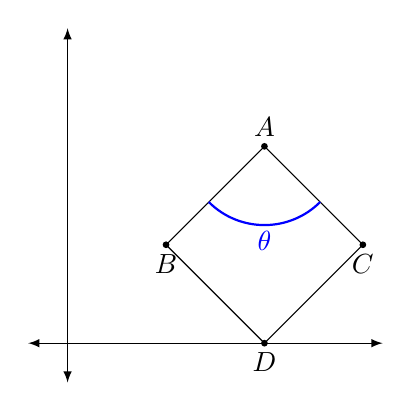
\begin{tikzpicture}[scale=0.5]
			% Coordinate axes
			\draw [<->] (-1,0) -- (8,0);
			\draw [<->] (0,-1) -- (0,8);

			% Points
			\coordinate (A) at (5,5);
			\coordinate (B) at (2.5,2.5);
			\coordinate (C) at (7.5,2.5);
			\coordinate (D) at (5,0);

			% Draw lines
			\draw (A) -- (B) -- (D) -- (C) -- cycle;

			% Draw points
			\filldraw (A) circle (2pt) node[above] {$A$};
			\filldraw (B) circle (2pt) node[below] {$B$};
			\filldraw (C) circle (2pt) node[below] {$C$};
			\filldraw (D) circle (2pt) node[below] {$D$};

			% Draw angle BAC
			\pic [draw, thick, blue, angle radius=1cm, angle eccentricity=1.2, "$\theta$"] {angle = B--A--C};
		\end{tikzpicture}
	\end{center}
	\[
		A'(0,0), \quad
		B'\left(-\frac{5}{2}, -\frac{5}{2}\right), \quad
		C'\left(\frac{5}{2}, -\frac{5}{2}\right), \quad
		D'(0, -5)
	\]

	\begin{center}
		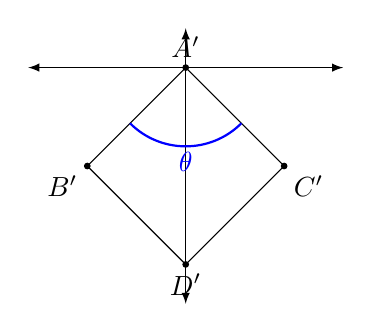
\begin{tikzpicture}[scale=0.5]
			% Coordinate axes
			\draw [<->] (-4,0) -- (4,0); % Adjusted to fit all points
			\draw [<->] (0,-6) -- (0,1);

			% Points
			\coordinate (A) at (0,0);
			\coordinate (B) at (-2.5,-2.5);
			\coordinate (C) at (2.5,-2.5);
			\coordinate (D) at (0,-5);

			% Draw lines
			\draw (A) -- (B) -- (D) -- (C) -- cycle;

			% Draw points
			\filldraw (A) circle (2pt) node[above] {$A'$};
			\filldraw (B) circle (2pt) node[below left] {$B'$};
			\filldraw (C) circle (2pt) node[below right] {$C'$};
			\filldraw (D) circle (2pt) node[below] {$D'$};

			% Draw angle B'A'C'
			\pic [draw, thick, blue, angle radius=1cm, angle eccentricity=1.2, "$\theta$"] {angle = B--A--C};
		\end{tikzpicture}
	\end{center}

	\[
		\vec{AB} = \vec{v_2} =
		\begin{bmatrix}
			-\frac{5}{2} \\
			-\frac{5}{2}
		\end{bmatrix}
		,
		\vec{AC} = \vec{v_1} =
		\begin{bmatrix}
			\frac{5}{2} \\
			-\frac{5}{2}
		\end{bmatrix}
	\]
	\[
		\vec{v_1}^T \vec{v_2} = -\frac{25}{4}+\frac{25}{4} = 0 =\left\lvert \vec{v_1} \right\rvert \left\lvert \vec{v_2}\right\rvert \cos(\theta)
	\]
	\[
		\therefore \theta = 90^\circ
	\]
}

\subsection{ERP's and Identity Matrices}


Let \( A'' \) be a matrix. Consider the augmented matrix:

\[
	\left[ A \mid I \right] : m \times 2m
\]

Perform a sequence of elementary row operations (ERPs) on \( A \) to turn it into the identity matrix \( I \):

\[
	E_p \dots E_2 E_1 A'' = B \left[ A \mid I \right] = \left[ BA \mid BI \right]
\]

where \( B \) is an \( m \times m \) matrix.

If we achieve \( BA = I \), then:

\[
	B = A^{-1}
\]

\qs{Thinklet}{
	Consider a set \( \mathcal{S}\) of vectors in \(\mathbb{R}^m\) who's tips form a straight line through the origin.	\\
	If we linearly combine a set of vectors in \(\mathcal{S}\), is the result guaranteed to be in \(\mathcal{S}\)?
}


\sol DUH

\chapter{Vector Spaces}

\dfn{Vector Space}{
	A vector space is a set of vectors in \(\mathbb{R}^m\) for which the following hold:

	\begin{enumerate}
		\item The set is closed under addition: that is, if \(\vec{v_1}, \vec{v_2}\) are both in the set, then \(\vec{v_1} + \vec{v_2}\) is also in the set.
		\item The set is closed under scalar multiplication: that is, if \(\vec{v}\) is in the set and \(c \in \mathbb{R}\), then \(c \vec{v}\) is also in the set.
	\end{enumerate}
}

\dfn{Basis of a Vector Space}{
	A basis for a vector space in \(\mathbb{R}^m\) is a set of independent vectors that span the vector space. The maximum number of vectors that could be in that basis is \( m \).\\
	\(m\) is the \textbf{dimension} of the vector space.
}

\ex{Examples of Vector Spaces}{
	\[
		\begin{array}{|c|c|c|}
			\hline
			\mathcal{S}                                                                                                                                                                                                                         & \text{Basis} & \text{Dimension} \\
			\hline
			\{ \vec{0} \}                                                                                                                                                                                                                       & \varnothing  & 0                \\
			\hline
			\left\{ \begin{bmatrix} a_1 \\ a_2 \\ \vdots \\ a_m \end{bmatrix} t \right\}                                                                                                                                                        &
			\left\{ \begin{bmatrix} a_1 \\ a_2 \\ \vdots \\ a_m \end{bmatrix} \right\}                                                                                                                                                          & 1                               \\
			\hline
			\left\{ \begin{bmatrix} a_1 \\ a_2 \\ \vdots \\ a_m \end{bmatrix} t_1 + \begin{bmatrix} b_1 \\ b_2 \\ \vdots \\ b_m \end{bmatrix} t_2 \right\}                                                                                      &
			\left\{ \begin{bmatrix} a_1 \\ a_2 \\ \vdots \\ a_m \end{bmatrix}, \begin{bmatrix} b_1 \\ b_2 \\ \vdots \\ b_m \end{bmatrix} \right\}                                                                                               & 2                               \\
			\hline
			\left\{ \sum_{i=1}^{k} \begin{bmatrix} a_{1i} \\ a_{2i} \\ \vdots \\ a_{mi} \end{bmatrix} t_i \right\}                                                                                                                              &
			\left\{ \begin{bmatrix} a_{11} \\ a_{21} \\ \vdots \\ a_{m1} \end{bmatrix}, \begin{bmatrix} a_{12} \\ a_{22} \\ \vdots \\ a_{m2} \end{bmatrix}, \ldots, \begin{bmatrix} a_{1k} \\ a_{2k} \\ \vdots \\ a_{mk} \end{bmatrix} \right\} & k                               \\
			\hline
		\end{array}
	\]
}

\section{Column Space}

\dfn{Column space of matrix \(A\)}{
	The \textit{column space} of an \( m \times n \) matrix \( A \), denoted as \( \text{Col}(A) \), is the subspace of \( \mathbb{R}^m \) spanned by the columns of \( A \). Formally,

	\[
		\text{Col}(A) = \text{span}(\mathbf{a}_1, \mathbf{a}_2, \dots, \mathbf{a}_n)
	\]

	where \( \mathbf{a}_1, \mathbf{a}_2, \dots, \mathbf{a}_n \) are the column vectors of \( A \). This means that \( \text{Col}(A) \) consists of all possible linear combinations of the columns of \( A \).

}

\section{Linear Combinations and Column Space}

\subsection{Basic Definitions and Concepts}

\dfn{Matrix Notation}{
An $m \times n$ matrix $A$ is a rectangular array of numbers with $m$ rows and $n$ columns. We can represent $A$ as a collection of column vectors:

\[
	A = [\vec{v}_1 \ \vec{v}_2 \ \dots \ \vec{v}_n]
\]

where each $\vec{v}_i$ is a vector in $\mathbb{R}^m$.
}

\dfn{Column Space (Col A)}{
The column space of a matrix $A$, denoted as Col $A$, is the set of all linear combinations of the columns of $A$.  Formally, if $A = [\vec{v}_1 \ \vec{v}_2 \ \dots \ \vec{v}_n]$, then

\[
	\text{Col } A = \text{span}\{\vec{v}_1, \vec{v}_2, \dots, \vec{v}_n\} = \{t_1\vec{v}_1 + t_2\vec{v}_2 + \dots + t_n\vec{v}_n \mid t_1, t_2, \dots, t_n \in \mathbb{R}\}
\]
}

\subsection{Dimension and Basis of the Column Space}

\qs{What is the dimension of Col A?}{
	The dimension of Col $A$ is equal to the number of pivot columns in the reduced row echelon form (REF) of $A$.
}
\sol{
	The dimension corresponds to the number of linearly independent columns in matrix $A$.
}

\qs{What is the basis for Col A?}{
	The basis for Col $A$ is formed by the column vectors of the \textbf{original} matrix $A$ that correspond to the pivot columns in the REF of $A$. These are referred to as the "basic columns."
}

\sol
\begin{enumerate}
	\item Find REF(A).
	\item Identify the pivot columns in REF(A).
	\item Select the corresponding columns from the \textbf{original* matrix A. These columns form the basis.}
\end{enumerate}


\subsection{Parametric Form of the Column Space}

\qs{What is the parametric form of Col A?}{
	If the basis for Col $A$ is $\{\vec{w}_1, \vec{w}_2, \dots, \vec{w}_k\}$, then the parametric form of any vector $\vec{v}$ in Col $A$ is given by:

	\[
		\vec{v} = t_1\vec{w}_1 + t_2\vec{w}_2 + \dots + t_k\vec{w}_k
	\]

	where $t_1, t_2, \dots, t_k$ are scalar parameters (real numbers).
}
\sol{
	This expresses any vector in the column space as a linear combination of the basis vectors.
}

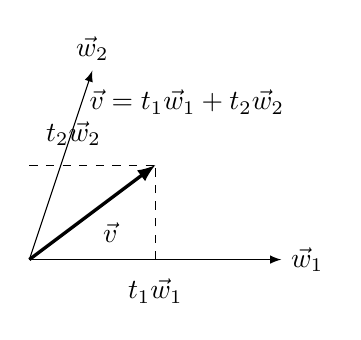
\begin{tikzpicture}[scale=0.8]
	\draw[->] (0,0) -- (4,0) node[right] {$\vec{w}_1$};
	\draw[->] (0,0) -- (1,3) node[above] {$\vec{w}_2$};
	\draw[->, very thick] (0,0) -- (2,1.5) node[midway, below right] {$\vec{v}$};
	\draw[dashed] (2,0) -- (2,1.5);
	\draw[dashed] (0,1.5) -- (2,1.5);
	\node at (2, -0.5) {$t_1\vec{w}_1$};
	\node at (0.7, 2) {$t_2\vec{w}_2$};

	\node at (2.5, 2.5) {$\vec{v} = t_1\vec{w}_1 + t_2\vec{w}_2$};
\end{tikzpicture}

\subsection{Geometry of the Column Space}

\qs{What is the geometry of Col A?}{
	The geometric interpretation of Col $A$ depends on its dimension:
	\begin{itemize}
		\item If dim(Col $A$) = 0, Col $A$ is a point (the origin, $\vec{0}$).
		\item If dim(Col $A$) = 1, Col $A$ is a line through the origin.
		\item If dim(Col $A$) = 2, Col $A$ is a plane through the origin.
		\item If dim(Col $A$) = 3, Col $A$ is a volume (all of $\mathbb{R}^3$) through the origin.
		\item In general, if  $A$ is an $m \times n$ matrix, and dim(Col $A$) = $k$,  Col $A$ is a k-dimensional subspace of $\mathbb{R}^m$.
	\end{itemize}
}
\sol{
	The dimension indicates the "degrees of freedom" or the number of independent directions spanned by the column vectors.
}

\subsection{Example}

\ex{Example Calculation}{
	Let
	\[
		A = \begin{bmatrix}
			1 & 2 & 3 \\
			3 & 2 & 1 \\
			2 & 4 & 6
		\end{bmatrix}
	\]

	Find the REF of $A$, the dimension of Col $A$, a basis for Col $A$, the parametric form of Col $A$, and the geometry of Col $A$.
}

\sol{
	First, find the reduced row echelon form (REF) of $A$:

	\[
		\text{REF}(A) = \begin{bmatrix}
			1 & 0  & -1 \\
			0 & -4 & -8 \\
			0 & 0  & 0
		\end{bmatrix} \rightarrow
		\begin{bmatrix}
			1 & 0 & -1 \\
			0 & 1 & 2  \\
			0 & 0 & 0
		\end{bmatrix}
	\]

	\begin{itemize}
		\item \textbf{Dimension of Col A:} The REF has two pivot columns (the first and second columns). Therefore, dim(Col $A$) = 2.

		\item \textbf{Basis for Col A:} The pivot columns in REF($A$) are the first and second columns.  We take the corresponding columns from the *original* matrix $A$ to form the basis:

		      \[
			      \text{Basis(Col } A) = \left\{ \begin{bmatrix} 1 \\ 3 \\ 2 \end{bmatrix}, \begin{bmatrix} 2 \\ 2 \\ 4 \end{bmatrix} \right\}
		      \]

		\item \textbf{Parametric Form of Col A:}  Any vector $\vec{v}$ in Col $A$ can be written as a linear combination of the basis vectors:

		      \[
			      \vec{v} = t_1 \begin{bmatrix} 1 \\ 3 \\ 2 \end{bmatrix} + t_2 \begin{bmatrix} 2 \\ 2 \\ 4 \end{bmatrix}
		      \]
		      where $t_1$ and $t_2$ are any real numbers.

		\item \textbf{Geometry of Col A:} Since dim(Col $A$) = 2, Col $A$ is a plane in $\mathbb{R}^3$ that passes through the origin.
	\end{itemize}
}

\section{Nullspace of a Matrix}

\dfn{Nullspace}{
	The nullspace of a matrix $A$, denoted by $\text{Nul } A$, is the set of all solutions to the homogeneous equation $A\vec{x} = \vec{0}$.
}

\nt{
	The solution space for $A\vec{x} = \vec{0}$ is a vector space. The nullspace of $A$ resides in $\mathbb{R}^n$, where $n$ is the number of columns of $A$.
}

\qs{Dimension of Nullspace}{
	What is the dimension of $\text{Nul } A$?
}
\sol{
	The dimension of $\text{Nul } A$ is equal to the number of free columns in the reduced row echelon form (RREF) of $A$.  We write this as $\text{Dim}(\text{Nul } A) = $ \# of free columns in RREF($A$).
}

\qs{Basis for Nullspace}{
	What is the basis for $\text{Nul } A$?
}
\sol{
	To find the basis for $\text{Nul } A$, we first find the RREF of $A$.  If the solution space of $A\vec{x} = \vec{0}$ is given by
	\[
		\vec{x} = t_1 \vec{w}_1 + t_2 \vec{w}_2 + \dots + t_k \vec{w}_k
	\]
	where $k$ is the number of free columns in RREF($A$), and $t_1, t_2, \dots, t_k$ are arbitrary scalars, then the basis of $\text{Nul } A$ is the set $\{\vec{w}_1, \vec{w}_2, \dots, \vec{w}_k\}$.
}
\qs{Parametric Form of Nullspace}{
	What is the parametric form of $\text{Nul } A$?
}
\sol{
	The parametric form of $\text{Nul } A$ is given by the linear combination of the basis vectors:
	\[
		\vec{v} = t_1 \vec{w}_1 + t_2 \vec{w}_2 + \dots + t_k \vec{w}_k
	\]
	where $\vec{w}_1, \vec{w}_2, ..., \vec{w}_k$ are the basis vector for the nullspace.
}

\ex{Example}{
	Let
	\[
		A = \begin{bmatrix}
			1 & 2 & 3 \\
			3 & 2 & 1 \\
			2 & 4 & 6
		\end{bmatrix}
	\]
	Find the nullspace, its dimension, basis, and the geometric interpretation.

	First, find the RREF of $A$:
	\[
		\text{REF}(A) = \begin{bmatrix}
			1 & 2  & 3  \\
			0 & -4 & -8 \\
			0 & 0  & 0
		\end{bmatrix}
	\]
	Further reducing to RREF:
	\[
		\text{RREF}(A) = \begin{bmatrix}
			1 & 0 & -1 \\
			0 & 1 & 2  \\
			0 & 0 & 0
		\end{bmatrix}
	\]

	\begin{itemize}
		\item The first column corresponds to a basic variable.
		\item The second column corresponds to a basic variable.
		\item The third column corresponds to a free variable.
	\end{itemize}

	The dimension of the nullspace is the number of free variables:
	\[
		\text{Dim}(\text{N}(A)) = 1
	\]

	To find the solution space for $A\vec{x} = \vec{0}$, we use the RREF:

	Let $\vec{x} = \begin{bmatrix} x_1 \\ x_2 \\ x_3 \end{bmatrix}$. The RREF gives us the following equations:
	\begin{align*}
		x_1 - x_3  & = 0 \\
		x_2 + 2x_3 & = 0
	\end{align*}
	$x_3$ is free. Let $x_3 = t_3$.  Then $x_1 = t_3$ and $x_2 = -2t_3$. So,
	\[
		\vec{x} = \begin{bmatrix}
			t_3 \\ -2t_3 \\ t_3
		\end{bmatrix} = t_3 \begin{bmatrix}
			1 \\ -2 \\ 1
		\end{bmatrix}
	\]

	Therefore, the basis for $\text{Nul } A$ is:
	\[
		\text{Basis}(\text{Nul } A) = \left\{ \begin{bmatrix} 1 \\ -2 \\ 1 \end{bmatrix} \right\}
	\]

	The geometry of $\text{Nul } A$ is a line in $\mathbb{R}^3$ passing through the origin and in the direction of the vector $\begin{bmatrix} 1 \\ -2 \\ 1 \end{bmatrix}$.

}
\begin{tikzpicture}[scale=1.5]
	\draw[->] (-0.5,0,0) -- (2,0,0) node[right] {$x_1$};
	\draw[->] (0,-1.5,0) -- (0,1,0) node[above] {$x_2$};
	\draw[->] (0,0,-0.5) -- (0,0,2) node[above left] {$x_3$};

	\draw[->, very thick] (0,0,0) -- (1,-2,1) node[midway,above right] {$\begin{bmatrix} 1 \\ -2 \\ 1 \end{bmatrix}$};
	\node[below] at (0,0,0) {Origin};
	\node[above] at (1,-2,1) {Line};

\end{tikzpicture}

\section{Row Space of a Matrix}

\dfn{Row Space}{
	The row space of a matrix $A$, denoted as Row $A$, is defined as the column space of the transpose of $A$, i.e., Row $A$ = Col $A^T$.
}

Let's consider a matrix $A$ and its transpose $A^T$:

\[
	A = \begin{bmatrix}
		- & r_1    & - \\
		- & r_2    & - \\
		  & \vdots &   \\
		- & r_m    & -
	\end{bmatrix}
	\qquad
	A^T = \begin{bmatrix}
		|     & |     &       & |     \\
		r_1^T & r_2^T & \dots & r_m^T \\
		|     & |     &       & |
	\end{bmatrix}
\]

Where $r_1, r_2, \dots, r_m$ represent the rows of matrix $A$. The rows of $A$ become the columns of $A^T$.

\nt{
	The row vectors $r_1, r_2, \dots, r_m$ live in $\mathbb{R}^n$.
}
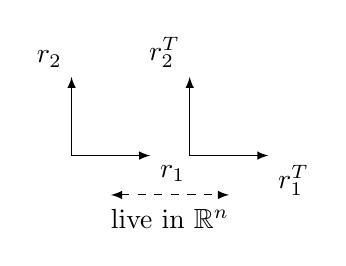
\begin{tikzpicture}
	\draw[->] (0,0) -- (1,0) node[anchor=north west] {$r_1$};
	\draw[->] (0,0) -- (0,1) node[anchor=south east] {$r_2$};
	\draw[->] (1.5,0) -- (2.5,0) node[anchor=north west] {$r_1^T$};
	\draw[->] (1.5,0) -- (1.5,1) node[anchor=south east] {$r_2^T$};

	\draw[<->,dashed] (0.5,-0.5)--(2,-0.5);

	\node at (1.25,-0.8) {live in $\mathbb{R}^n$};
\end{tikzpicture}

\section{Dimension and Basis of Row Space}

\qs{What is the dimension of Row $A$?}{
	What is the dimension of the row space of a matrix $A$?
}

\sol{
	The dimension of Row $A$ is equal to the number of pivots in the row echelon form (REF) of $A$. It is also equal to the number of pivots in the REF of $A^T$.
	\[
		\text{Dim(Row } A) = \text{\# pivots in REF}(A) = \text{\# pivots in REF}(A^T)
	\]
}
\qs{What is the Basis of Row A}{
	How to find the basis for the Row Space of A
}

\sol{
	\begin{enumerate}
		\item Identify all the rows of REF($A$) that have pivots.
		\item The basis vectors for Row $A$ are:
		      \begin{itemize}
			      \item Vectors corresponding to rows (with pivots in REF($A$)) of $A$.
		      \end{itemize}
		      OR
		      \begin{itemize}
			      \item Vectors corresponding to rows (with pivots in REF($A$)) of REF($A$).
		      \end{itemize}
		      OR
		      \begin{itemize}
			      \item Vectors corresponding to rows (with pivots in REF($A$)) of RREF($A$).
		      \end{itemize}
	\end{enumerate}
}

\ex{Example: Finding the Basis and Dimension}{
	Let
	\[
		A = \begin{bmatrix}
			1 & 2 & 3 \\
			2 & 4 & 6 \\
			1 & 2 & 3
		\end{bmatrix}
	\]
	Find the dimension and a basis for Row $A$.
}

\sol{
	First, find the REF of $A$:
	\[
		\text{REF}(A) = \begin{bmatrix}
			1 & 2 & 3 \\
			0 & 0 & 0 \\
			0 & 0 & 0
		\end{bmatrix}
	\]
	The REF of $A$ has one pivot (in the first row).

	Dimension of Row $A$:
	\[
		\text{Dim(Row } A) = 1
	\]

	Basis for Row $A$:
	\begin{itemize}
		\item Using rows of $A$ with pivots in REF($A$): {[1 2 3]}
		\item Using rows of REF($A$) with pivots: {[1 2 3]}
	\end{itemize}
}
\begin{algorithm}[H]
	\KwIn{Matrix $A$}
	\KwOut{Dimension of Row $A$, Basis of Row $A$}
	\SetAlgoLined
	\SetNoFillComment

	\tcc{Compute the Row Echelon Form (REF) of A}
	$REF\_A$ $\leftarrow$ REF($A$);

	\tcc{Count the number of pivots in REF(A)}
	$num\_pivots$ $\leftarrow$ Number of pivots in $REF\_A$;

	\tcc{The dimension of Row A is the number of pivots}
	$dim\_row\_A$ $\leftarrow$ $num\_pivots$;

	\tcc{Initialize an empty set to store basis vectors}
	$basis\_row\_A$ $\leftarrow$ $\emptyset$;

	\tcc{Identify rows with pivots in REF(A)}
	\ForEach{row $r$ in $REF\_A$}{
		\If{row $r$ has a pivot}{

			\tcc{Add corresponding row from original matrix A to basis}
			Let $r'$ be the corresponding row in matrix $A$.
			$basis\_row\_A$ $\leftarrow$ $basis\_row\_A$ $\cup$ \{$r'$\};
		}
	}
	\Return{$dim\_row\_A$, $basis\_row\_A$};
	\caption{Finding Dimension and Basis of Row Space}
\end{algorithm}

\chapter{Properties of Matrices}

\section{Determinant of a Square Matrix}
Consider a square Matrix
\[
	A: \, m \times m
\]
If
\[
	A^{-1} exists \Leftrightarrow \dim(Col(A)) = \dim(Row(A)) = m
\]
\[
	\therefore Rank(A) = m \, \text{and} \, \text{Nul}(A) = \{0\}
\]
And most importantly, since the columns of A are linearly independent,
\[
	det(ref(A)) \neq 0
\]


\vspace{0.5cm}
To make $\text{REF}(A)$ unique for $A$, we require that in constructing $\text{REF}(A)$, we follow three rules:

\begin{enumerate}
	\item Use the ``REPLACE'' ERP freely.
	\item When using the ``SWAP'' ERP, apply the ``SCALE'' ERP to one of the rows by $-1$.
	\item Don't use the ``SCALE'' ERP for any other purpose than the one in Rule 2.
\end{enumerate}

\subsection{Cofactor Algorithm for Computing Determinant}


Given a square matrix \( A = [a_{ij}] \) of size \( n \times n \), the determinant can be computed by expanding along any row \( i \) (where \( 1 \leq i \leq n \)) as follows:

\begin{enumerate}
	\item \textbf{Base Case}: If \( n = 1 \), then \( \det(A) = a_{11} \).

	\item \textbf{Recursive Case}: For \( n > 1 \):
	      \[
		      \det(A) = \sum_{j=1}^n (-1)^{i+j} \, a_{ij} \, \det(M_{ij}),
	      \]
	      where:
	      \begin{itemize}
		      \item \( M_{ij} \) is the \textbf{minor matrix} obtained by deleting row \( i \) and column \( j \) from \( A \),
		      \item \( (-1)^{i+j} \, \det(M_{ij}) \) is the \textbf{cofactor} of the element \( a_{ij} \).
	      \end{itemize}
\end{enumerate}

\noindent \textbf{Steps}:
\begin{itemize}
	\item Choose a row \( i \) (commonly the first row, \( i = 1 \), but any row works).
	\item For each element \( a_{ij} \) in row \( i \):
	      \begin{itemize}
		      \item Compute the minor \( M_{ij} \).
		      \item Recursively calculate \( \det(M_{ij}) \).
		      \item Multiply \( a_{ij} \), \( (-1)^{i+j} \), and \( \det(M_{ij}) \).
	      \end{itemize}
	\item Sum the results for all columns \( j \) in row \( i \).
\end{itemize}

Say \(B\) which has the Form

\[
	\begin{bmatrix}
		a_1 & a_2 & \dots \\
		b_1 & b_2 & \dots \\
	\end{bmatrix}
\]

And delimits an area in \( \mathbb{R}^2 \), then the absolute value of the determinant of a matrix \(A\) which applies a transformation to \(B\) gives the scaling of the area of \(B\)

\subsection{Properties of Determinants}


\begin{multicols}{2}
	\begin{itemize}
		\item \(det(A \cdot B) = det(A) \cdot det(B)\)
		\item \(det(A^{-1}) = \frac{1}{det(A)}\)
		\item \(det(A^T) = det(A)\)
		\item \(det(I)=1\)
		\item \(det(E_{REPLACE} \cdot A) = det(A)\)
		\item \(det(E_{SCALE= \alpha} \cdot A) = \alpha \cdot det(A)\)
		\item \(det(A) = 0 \Leftrightarrow det(REF(A))= 0\)
	\end{itemize}
\end{multicols}

\section{EigenVectors and EigenValues}

Given \(A \in \mathbb{R}^{n \times n}\)

\[
	A \vec{x} = \vec{0} \leftarrow \vec{x} \in Null(A)
\]

Can rewrite As

\[
	A \vec{x} = 0 \vec{x}
\]

Generalise

\[
	A \vec{x} = \lambda \vec{x}
\]

where the solution for \(\vec{x}\) also defines a vector space, called an \textbf{EigenSpace}, where any vector in this space is called and \textbf{EigenVector}, and has a corresponding value of \(\lambda\) called an \textbf{EigenValue}.

\ex{Eigenvectors}{
	\[
		A =
		\begin{bmatrix}
			-2 & 0 \\
			0  & 3
		\end{bmatrix}
	\]
	is \(\begin{bmatrix} 2\\2 \end{bmatrix}\) an eigenvector for \(A\)?

	\[
		\begin{bmatrix}
			-2 & 0 \\
			0  & 3
		\end{bmatrix}
		\begin{bmatrix} 2\\2 \end{bmatrix}
		=
		\begin{bmatrix}
			-4 \\
			6
		\end{bmatrix}
		=
		\lambda
		\begin{bmatrix} 2\\2 \end{bmatrix}
	\]
	No such Lambda, therefore not eigenvector, but
	\[
		\begin{bmatrix}
			-2 & 0 \\
			0  & 3
		\end{bmatrix}
		\begin{bmatrix}
			2 \\0
		\end{bmatrix}
		=
		\begin{bmatrix}
			-4 \\0
		\end{bmatrix}
		=
		-2
		\begin{bmatrix}
			2 \\0
		\end{bmatrix}
	\]

	So \(\lambda = -2\) is the EigenValue for the EigenVector that is \(\begin{bmatrix} 2\\0 \end{bmatrix}\)

}

\section*{Eigenvectors and Eigenvalues}

\dfn{Eigenvector and Eigenvalue}{
	Let $A$ be an $n \times n$ matrix. A non-zero vector $\vec{x}$ is an eigenvector of $A$ if there exists a scalar $\lambda$ (called an eigenvalue) such that:
	\[A\vec{x} = \lambda\vec{x}\]
}

\nt{
	The geometric interpretation of $A\vec{x} = \lambda\vec{x}$ is that applying the transformation represented by $A$ to the eigenvector $\vec{x}$ results in a vector that is simply a scaled version of $\vec{x}$.  The direction is either preserved (if $\lambda > 0$), reversed (if $\lambda < 0$), or the vector becomes the zero vector (if $\lambda = 0$).  Crucially, $\vec{x}$ *cannot* be the zero vector, but $\lambda$ can be.
}

\ex{Rotation Matrix}{
	Consider a rotation matrix $A$ in 2D that rotates vectors by 45 degrees counterclockwise:

	\[A = \begin{bmatrix} \cos(45^\circ) & -\sin(45^\circ) \\ \sin(45^\circ) & \cos(45^\circ) \end{bmatrix} = \begin{bmatrix} \frac{\sqrt{2}}{2} & -\frac{\sqrt{2}}{2} \\ \frac{\sqrt{2}}{2} & \frac{\sqrt{2}}{2} \end{bmatrix}\]

	\begin{tikzpicture}
		\draw[->] (-1.5,0) -- (1.5,0) node[right] {$x_1$};
		\draw[->] (0,-1.5) -- (0,1.5) node[above] {$x_2$};
		\draw[->, thick] (0,0) -- (1,0) node[midway, below] {$\vec{x}$};
		\draw[->, thick, blue] (0,0) -- (0,1) node[midway, left] {$A\vec{x}$};
		\draw (0.5,0) arc (0:90:0.5);
		\node at (0.3,0.3) {$45^\circ$};
	\end{tikzpicture}

	This matrix $A$ has *no* real eigenvectors (and thus no real eigenvalues).  Applying $A$ to any non-zero vector $\vec{x}$ will *always* rotate it; there's no non-zero vector that will simply be scaled by $A$. The resulting vector $A\vec{x}$ will never have the same (or opposite) direction as the original $\vec{x}$.
}

\ex{Horizontal Shear and Stretch}{
	Consider the matrix:

	\[A = \begin{bmatrix} 2 & 0.5 \\ 0 & 1 \end{bmatrix}\]

	This matrix represents a horizontal shear and stretch.  Let's visualize its effect on a unit square:

	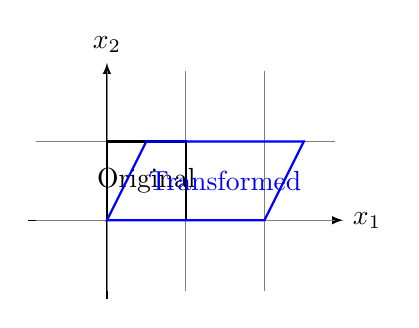
\begin{tikzpicture}
		\draw[->] (-1,0) -- (3,0) node[right] {$x_1$};
		\draw[->] (0,-1) -- (0,2) node[above] {$x_2$};

		\draw[step=1cm,gray,very thin] (-0.9,-0.9) grid (2.9,1.9);

		% Original Square
		\draw[thick] (0,0) -- (1,0) -- (1,1) -- (0,1) -- cycle;
		\node at (0.5, 0.5) {Original};

		% Transformed Square
		\draw[thick, blue] (0,0) -- (2,0) -- (2.5,1) -- (0.5,1) -- cycle;
		\node[blue] at (1.5, 0.5) {Transformed};
	\end{tikzpicture}

	\begin{itemize}
		\item Vectors along the $x_1$-axis (of the form $\alpha \begin{bmatrix} 1 \\ 0 \end{bmatrix}$) are stretched by a factor of 2, but their direction remains unchanged.
		\item Vectors along the $x_2$-axis (of the form $\alpha \begin{bmatrix} 0 \\ 1 \end{bmatrix}$) are sheared horizontally by 0.5 units, but their vertical component is unchanged.
		\item  Consider a general vector $\begin{bmatrix} \alpha \\ \beta \end{bmatrix}$. Applying the transformation yields $A\begin{bmatrix} \alpha \\ \beta \end{bmatrix} = \begin{bmatrix} 2\alpha + 0.5\beta \\ \beta \end{bmatrix}$.
	\end{itemize}

	Let's find the eigenvectors and eigenvalues for this matrix.

	\begin{itemize}
		\item For vectors along the $x_1$ axis:
		      \[A \begin{bmatrix} \alpha \\ 0 \end{bmatrix} = \begin{bmatrix} 2 & 0.5 \\ 0 & 1 \end{bmatrix} \begin{bmatrix} \alpha \\ 0 \end{bmatrix} = \begin{bmatrix} 2\alpha \\ 0 \end{bmatrix} = 2 \begin{bmatrix} \alpha \\ 0 \end{bmatrix}\]
		      So, $\begin{bmatrix} \alpha \\ 0 \end{bmatrix}$ is an eigenvector with eigenvalue $\lambda = 2$.

		\item For vectors along the $x_2$ axis, we might *think* they are eigenvectors, but let's check:
		      \[A \begin{bmatrix} 0 \\ \alpha \end{bmatrix} = \begin{bmatrix} 2 & 0.5 \\ 0 & 1 \end{bmatrix} \begin{bmatrix} 0 \\ \alpha \end{bmatrix} = \begin{bmatrix} 0.5\alpha \\ \alpha \end{bmatrix} = \alpha \begin{bmatrix} 0.5 \\ 1 \end{bmatrix}\]
		      This is *not* a scalar multiple of the original vector $\begin{bmatrix} 0 \\ \alpha \end{bmatrix}$.  So, vectors along the $x_2$ axis are *not* eigenvectors.

		\item Now consider the case where the transformed vector is $\alpha$ times the original:
		      \[\begin{bmatrix} 2 & 0.5 \\ 0 & 1 \end{bmatrix} \begin{bmatrix} -0.5\alpha \\ \alpha \end{bmatrix} =
			      \begin{bmatrix} -1\alpha + 0.5\alpha \\ \alpha \end{bmatrix} =
			      \begin{bmatrix} -0.5\alpha \\ \alpha \end{bmatrix} = 1 * \begin{bmatrix} -0.5\alpha \\ \alpha \end{bmatrix}\]
		      So $\begin{bmatrix} -0.5\alpha \\ \alpha \end{bmatrix}$ is an eigenvector corresponding to eigenvalue 1.

	\end{itemize}
}

\subsection*{Finding Eigenvalues and Eigenvectors}

\thm{Finding Eigenvalues}{
	To find the eigenvalues of a matrix $A$, we solve the characteristic equation:
	\[\det(A - \lambda I) = 0\]
	where $I$ is the identity matrix of the same size as $A$.
}
\begin{proof}
	We start with the definition $A\vec{x} = \lambda\vec{x}$.  Rearranging, we get:

	\[A\vec{x} - \lambda\vec{x} = \vec{0}\]
	\[A\vec{x} - \lambda I\vec{x} = \vec{0}\]
	\[(A - \lambda I)\vec{x} = \vec{0}\]

	Let $B = A - \lambda I$.  We have $B\vec{x} = \vec{0}$.  We are looking for non-zero vectors $\vec{x}$ that satisfy this equation.

	\begin{itemize}
		\item If $B$ is invertible (i.e., $\det(B) \neq 0$), then the only solution is $\vec{x} = \vec{0}$.  But eigenvectors are *non-zero* by definition.  Therefore, we must have $\det(B) = 0$.
		\item If $\det(B) = 0$, then $B$ is *not* invertible, and the system $B\vec{x} = \vec{0}$ has infinitely many solutions (i.e., a non-trivial null space). These non-zero solutions are the eigenvectors.
	\end{itemize}

	Therefore, to find the eigenvalues $\lambda$, we must solve $\det(A - \lambda I) = 0$.
\end{proof}

\ex{Finding Eigenvalues (Continued)}{
	Let's go back to our example:
	\[A = \begin{bmatrix} 2 & 0.5 \\ 0 & 1 \end{bmatrix}\]
	We form $B = A - \lambda I$:
	\[B = \begin{bmatrix} 2 & 0.5 \\ 0 & 1 \end{bmatrix} - \lambda \begin{bmatrix} 1 & 0 \\ 0 & 1 \end{bmatrix} = \begin{bmatrix} 2-\lambda & 0.5 \\ 0 & 1-\lambda \end{bmatrix}\]
	Now we find the determinant of $B$:
	\[\det(B) = (2-\lambda)(1-\lambda) - (0.5)(0) = (2-\lambda)(1-\lambda)\]
	Setting $\det(B) = 0$, we get:
	\[(2-\lambda)(1-\lambda) = 0\]
	This gives us the eigenvalues $\lambda_1 = 2$ and $\lambda_2 = 1$.
}

\subsection*{Finding Eigenvectors}
\begin{algorithm}[H]
	\KwIn{A matrix $A$}
	\KwOut{Eigenvalues and corresponding eigenvectors of $A$}
	\SetAlgoLined
	\SetNoFillComment
	\vspace{3mm}
	Calculate the characteristic polynomial: $\det(A - \lambda I)$\;
	Solve the characteristic equation $\det(A-\lambda I) = 0$ to find the eigenvalues $\lambda_i$\;
	\For{each eigenvalue $\lambda_i$}{
		Form the matrix $B_i = A - \lambda_i I$\;
		Solve the homogeneous system $B_i \vec{x} = \vec{0}$ to find the eigenvectors corresponding to $\lambda_i$\;
		The solution set will typically involve free variables.  Express the eigenvectors in terms of these free variables.\;
	}
	\Return The eigenvalues $\lambda_i$ and their corresponding eigenvectors.
	\caption{Finding Eigenvalues and Eigenvectors}
\end{algorithm}

\ex{Finding Eigenvectors (Continued)}{
	We found the eigenvalues $\lambda_1 = 2$ and $\lambda_2 = 1$ for the matrix $A = \begin{bmatrix} 2 & 0.5 \\ 0 & 1 \end{bmatrix}$.  Now let's find the eigenvectors.

	\begin{itemize}
		\item For $\lambda_1 = 2$:
		      \[B_1 = A - 2I = \begin{bmatrix} 2-2 & 0.5 \\ 0 & 1-2 \end{bmatrix} = \begin{bmatrix} 0 & 0.5 \\ 0 & -1 \end{bmatrix}\]
		      We solve $B_1\vec{x} = \vec{0}$:
		      \[\begin{bmatrix} 0 & 0.5 \\ 0 & -1 \end{bmatrix} \begin{bmatrix} x_1 \\ x_2 \end{bmatrix} = \begin{bmatrix} 0 \\ 0 \end{bmatrix}\]
		      Row reducing (although not strictly necessary here, we do it for demonstration):
		      \[\begin{bmatrix} 0 & 0.5 \\ 0 & -1 \end{bmatrix} \rightarrow
			      \begin{bmatrix} 0 & 1 \\ 0 & -1 \end{bmatrix} \rightarrow
			      \begin{bmatrix} 0 & 1 \\ 0 & 0 \end{bmatrix}\]
		      This gives us $x_2 = 0$, and $x_1$ is free.  Let $x_1 = t_1$. Then the eigenvector is:
		      \[\vec{x} = \begin{bmatrix} t_1 \\ 0 \end{bmatrix} = t_1 \begin{bmatrix} 1 \\ 0 \end{bmatrix}\]

		\item For $\lambda_2 = 1$:
		      \[B_2 = A - I = \begin{bmatrix} 2-1 & 0.5 \\ 0 & 1-1 \end{bmatrix} = \begin{bmatrix} 1 & 0.5 \\ 0 & 0 \end{bmatrix}\]
		      We solve $B_2\vec{x} = \vec{0}$:
		      \[\begin{bmatrix} 1 & 0.5 \\ 0 & 0 \end{bmatrix} \begin{bmatrix} x_1 \\ x_2 \end{bmatrix} = \begin{bmatrix} 0 \\ 0 \end{bmatrix}\]
		      This system is already in row-echelon form. We have $x_1 + 0.5x_2 = 0$, so $x_1 = -0.5x_2$.  $x_2$ is free. Let $x_2 = t_2$. Then $x_1 = -0.5t_2$, and the eigenvector is:
		      \[\vec{x} = \begin{bmatrix} -0.5t_2 \\ t_2 \end{bmatrix} = t_2 \begin{bmatrix} -0.5 \\ 1 \end{bmatrix}\]
	\end{itemize}
}

\section{Properties of Eigenvectors}

\dfn{Dimension of eigenspace}{

	When an eigenvalue repeats \(k\) times,
	\[
		1 \leq dim(\text{eigenspace for that eigenvalue}) \leq k
	\]

}

\ex{Example 1 of this property}{
	\[
		A=
		\begin{bmatrix}
			1 & 0 & 0 \\
			0 & 1 & 0 \\
			0 & 0 & 1
		\end{bmatrix}
	\]
	\[
		A-\lambda I =
		\begin{bmatrix}
			1 - \lambda & 0           & 0           \\
			0           & 1 - \lambda & 0           \\
			0           & 0           & 1 - \lambda
		\end{bmatrix}
	\]
	\[
		\det(A- \lambda I) = (I1-\lambda)^3
	\]
	\[
		\lambda_1 = 1, \lambda_2 = 1, \lambda_3 = 1, k=3
	\]
	\[
		\lambda_1 \text{repeats} 3 (=k) \text{times}
	\]
	And the eigenspace for$ \lambda_1 = 1$ is
	\[
		A-\lambda_1 I =
		\begin{bmatrix}
			0 & 0 & 0 \\
			0 & 0 & 0 \\
			0 & 0 & 0
		\end{bmatrix}
	\]
	therefore the eigenspace is
	\[
		\left\{ t_1 \begin{bmatrix}
			1 \\ 0 \\ 0
		\end{bmatrix} + t_2 \begin{bmatrix}
			0 \\ 1 \\ 0
		\end{bmatrix} + t_3 \begin{bmatrix}
			0 \\ 0 \\ 1
		\end{bmatrix} : t_1, t_2, t_3 \in \mathbb{R} \right\}
	\]
}

\ex{Example 2 of this property}{
	\[
		A=
		\begin{bmatrix}
			1 & 0.5 \\
			0 & 1
		\end{bmatrix}
	\]
	\[
		\det(A- \lambda I) = (I1-\lambda)^3
	\]
	\[
		(1-\lambda)^2 -(0.5)(0) = 0
	\]
	\[
		\lambda_1 = 1, \lambda_2 = 1, k=2
	\]
	Therefore the eigenspace is
	\[
		A-\lambda_1 I =
		\begin{bmatrix}
			0 & 0.5 \\
			0 & 0
		\end{bmatrix}
		\xrightarrow{R_1 = 2R_1}
		\begin{bmatrix}
			0 & 1 \\
			0 & 0
		\end{bmatrix}
	\]
	Therefore the eigenspace for \(\lambda = 1\) is
	\[
		\left\{ t_1 \begin{bmatrix}
			1 \\ 0
		\end{bmatrix} : t_1 \in \mathbb{R} \right\}
	\]
	\[
		\therefore dim(\text{eigenspace for } \lambda = 1) = 1 \leq k = 2
	\]
}
\dfn{Dominant Eigenvector}{
	An eigenvector whose eigenvalue (among all eigenvalues for some \(A : m \times m\)) has the largest magnitude (\(|\lambda|\)) gives the direction along which an initial blob of points is stretched the most.
}

\ex{Dominant Eigenvector Example}{
	A=
	\[
		\begin{bmatrix}
			2 & 4 \\
			3 & 3
		\end{bmatrix}
	\]
	\[
		\det(A-\lambda I) = (2-\lambda)(3-\lambda) - 4*3 = 0
	\]
	\[
		\therefore \lambda_1 = 6, \lambda_2 = -1
	\]
	Eigenspace for largest magnitude of eigenvalue \(\lambda_1 = 6\)
	\[
		A =
		\begin{bmatrix}
			-4 & 4  \\
			3  & -3
		\end{bmatrix}
		\xrightarrow{R_2 = R_2 + \frac{3}{4}R_1}
		\begin{bmatrix}
			-4 & 4 \\
			0  & 0
		\end{bmatrix}
		\xrightarrow{R_1 = -\frac{1}{4}R_1}
		\begin{bmatrix}
			1 & -1 \\
			0 & 0
		\end{bmatrix}
	\]
	\[
		\therefore \vec{v}_1 = t_2 \begin{bmatrix}
			1 \\ 1
		\end{bmatrix}
	\]
	and the eigenspace for \(\lambda_1 = 6\) is
	\[
		\left\{ t \begin{bmatrix}
			1 \\ 1
		\end{bmatrix} : t \in \mathbb{R} \right\}
	\]

	Now apply the transformation to a set of points (unit square)

	\[
		\begin{bmatrix}
			1 & 0 \\
			0 & 1
		\end{bmatrix}
		\begin{bmatrix}
			2 & 3 \\
			4 & 3
		\end{bmatrix}
		=
		\begin{bmatrix}
			2 & 3 \\
			4 & 3
		\end{bmatrix}
	\]

	Visually represented this looks like this

	\begin{tikzpicture}[scale=1.2,>=stealth]
		%--- Original Coordinate System ---
		\draw[->] (-1.5,0) -- (2,0) node[right] {$x$};
		\draw[->] (0,-1.5) -- (0,2) node[above] {$y$};
		% Define the original square vertices
		\coordinate (P) at (0,0);
		\coordinate (Q) at (1,0);
		\coordinate (R) at (1,1);
		\coordinate (S) at (0,1);
		% Draw the original square
		\draw[step=1, gray, very thin] (P) grid (R);
		\draw[thick] (P) -- (Q) -- (R) -- (S) -- cycle;
		% Label original square vertices
		\node[below left] at (P) {$P(0,0)$};
		\node[below right] at (Q) {$Q(1,0)$};
		\node[above right] at (R) {$R(1,1)$};
		\node[above left] at (S) {$S(0,1)$};
		\node at ($(P)!0.5!(S)+(-0.5,0)$) {Original};

		%--- Transformation Arrow ---
		\draw[->, thick] (2.2,0.5) -- (3.2,0.5) node[midway, above] {$A$};

		%--- Transformed Coordinate System ---
		% Apply the linear transformation A = [3 \, 1; 0 \, 2]
		\begin{scope}[shift={(4.5,0)}]
			\draw[->] (-1.5,0) -- (3,0) node[right] {$x'$};
			\draw[->] (0,-1.5) -- (0,3) node[above] {$y'$};
			% Define transformed square vertices (using given coordinates)
			\coordinate (A) at (0,0);
			\coordinate (B) at (4,3);
			\coordinate (C) at (6,6);
			\coordinate (D) at (2,3);
			\draw[thick, blue] (A) -- (B) -- (C) -- (D) -- cycle;
			% Label transformed square vertices
			\node[below left] at (A) {$A'(0,0)$};
			\node[below right] at (B) {$B'(4,3)$};
			\node[above right] at (C) {$C'(6,6)$};
			\node[above left] at (D) {$D'(2,3)$};
			\node at ($(A)!0.5!(D)+(-0.5,0)$) {Transformed};

			% Transform the vector <1,1>:
			% A(1,1) = (3*1+1*1,\,0*1+2*1) = (4,2)
			\draw[->, ultra thick, red] (0,0) -- (1,1)
			node[above right] {$\langle 1,1\rangle$};
		\end{scope}
	\end{tikzpicture}

}
\ex{Dominant Eigenvector Example 2}{
	Consider
	\[
		A=\begin{bmatrix}3 & 1\\[4pt] 0 & 2\end{bmatrix}.
	\]
	The eigenvalues come from
	\[
		\det(A-\lambda I)=(3-\lambda)(2-\lambda)=0,
	\]
	so \(\lambda_1=3\) and \(\lambda_2=2\). The dominant eigenvalue is \(3\). To find its eigenvector, solve
	\[
		(A-3I)\vec{v}=\begin{bmatrix}0 & 1\\[4pt] 0 & -1\end{bmatrix}\begin{bmatrix}v_1\\v_2\end{bmatrix}=\vec{0}.
	\]
	The first row gives \(v_2=0\); choosing \(v_1=1\) yields
	\[
		\vec{v}_1=\begin{bmatrix}1\\0\end{bmatrix}.
	\]
	This indicates that the largest stretch occurs in the horizontal direction.

	\medskip
	\textbf{Transformation on a set of points:}

	Consider the original set of points
	\[
		\mathcal{P}=\{(x,y)\mid -1\le x\le 1,\; -0.5\le y\le 0.5\}.
	\]
	Under the transformation \(A\), each point \((x,y)\) is mapped to
	\[
		(x',y')=(3x+y,\;2y).
	\]
	The four corners transform as follows:
	\begin{itemize}
		\item \((-1,-0.5)\) maps to \((3(-1)+(-0.5),\;2(-0.5))=(-3.5,\;-1)\).
		\item \((1,-0.5)\) maps to \((3(1)+(-0.5),\;2(-0.5))=(2.5,\;-1)\).
		\item \((1,0.5)\) maps to \((3(1)+(0.5),\;2(0.5))=(3.5,\;1)\).
		\item \((-1,0.5)\) maps to \((3(-1)+(0.5),\;2(0.5))=(-2.5,\;1)\).
	\end{itemize}
	Thus, the image of \(\mathcal{P}\) is the quadrilateral
	\[
		\mathcal{P}'=\{(x',y')\}
	\]
	with vertices at \((-3.5,-1)\), \((2.5,-1)\), \((3.5,1)\), and \((-2.5,1)\).

	\medskip
	\textbf{Diagram:}

	\begin{center}
		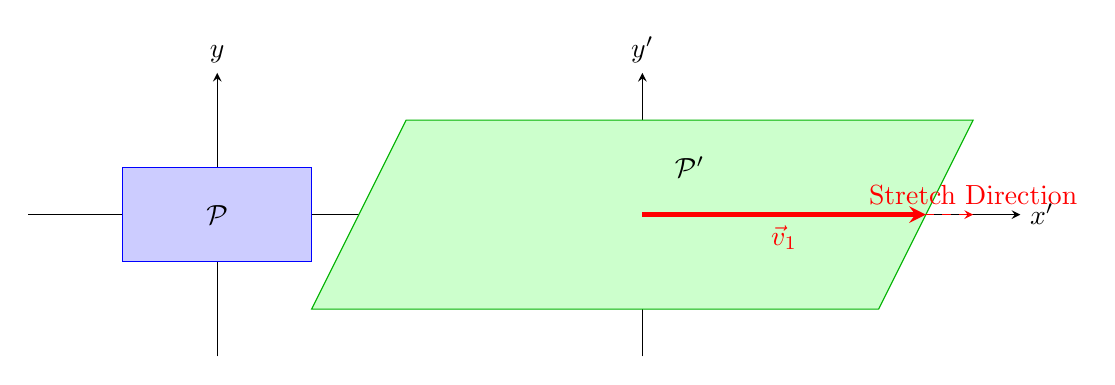
\begin{tikzpicture}[scale=1.2,>=stealth]
			% Left coordinate system: original space
			\draw[->] (-2,0) -- (2,0) node[right] {$x$};
			\draw[->] (0,-1.5) -- (0,1.5) node[above] {$y$};
			\filldraw[fill=blue!20, draw=blue] (-1,-0.5) rectangle (1,0.5);
			\node at (0,0) {$\mathcal{P}$};

			% Arrow indicating transformation
			\draw[->, thick] (2.2,0) -- (3.3,0) node[midway, above] {Transformation};

			% Right coordinate system: transformed space
			\begin{scope}[shift={(4.5,0)}]
				\draw[->] (-3.5,0) -- (4,0) node[right] {$x'$};
				\draw[->] (0,-1.5) -- (0,1.5) node[above] {$y'$};
				\coordinate (A) at (-3.5,-1);
				\coordinate (B) at (2.5,-1);
				\coordinate (C) at (3.5,1);
				\coordinate (D) at (-2.5,1);
				\filldraw[fill=green!20, draw=green!70!black] (A) -- (B) -- (C) -- (D) -- cycle;
				\node at (0.5,0.5) {$\mathcal{P}'$};

				% Draw dominant eigenvector arrow
				\draw[->, ultra thick, red] (0,0) -- (3,0) node[midway, below] {\(\vec{v}_1\)};
				\draw[->, dashed, red] (3,0) -- (3.5,0) node[above] {Stretch Direction};
			\end{scope}
		\end{tikzpicture}
	\end{center}
}

\dfn{Eigenvalues of Triangular Matrices}{
	The elements on the main diagonal of a triangular matrix are the eigenvalues of that matrix.
}

\ex{EigenValues of Triangular matricies example}{
	\[
		A=
		\begin{bmatrix}
			1 & 2 & 3 \\
			0 & 4 & 5 \\
			0 & 0 & 6
		\end{bmatrix}
	\]
	\[
		\det(A-\lambda I) = (1-\lambda)(4-\lambda)(6-\lambda)
	\]
	\[
		\lambda_1 = 1, \lambda_2 = 4, \lambda_3 = 6
	\]
	\[
		\text{Eigenvalues of } A = \{1,4,6\}
	\]
}

\dfn{Number of Distinct EigenValues}{
	The number of distinct eigenvalues of a matrix \(A: m \times m\) is \(\leq m\)
}
\dfn{Eigenvalues and Determinant}{
	For a matrix \(A: m \times m\)
	\[
		\det(A) = \lambda_1 \cdot \lambda_2 \cdot  \dots \cdot \lambda_m
	\]
	Proof:
	\[
		dat(A - \lambda I) = \pm \lambda^m + a_{m-1} \lambda^{m-1} + \dots + a_1 \lambda + a_0
	\]
	where the \(\pm\) follows
	\[
		\begin{cases}
			+1, & m \% 2 = 0 \\
			-1, & m \% 2 = 1 \\
		\end{cases}
	\]
	\[
		\therefore
		|A-\lambda I| = 
		\begin{cases}
			\lambda^m - a_{m-1} \lambda^{m-1} + \dots - a_1 \lambda + a_0, & m \% 2 = 0 \\
			-\lambda^m + a_{m-1} \lambda^{m-1} - \dots + a_1 \lambda - a_0, & m \% 2 = 1 \\
		\end{cases}
	\]
	Set \(\lambda = 0\)
	\[
		|A| = 
		\begin{cases}
			\lambda_1, \lambda_2, \dots, \lambda_m, & m \% 2 = 0 \\
			\lambda_1, \lambda_2, \dots, \lambda_m, & m \% 2 = 0 \\	
		\end{cases}
	\]
}


\dfn{Non-invertible Square matrix}{
	For a non-invertible (singular) square matrix \(A: m \times m\), the determinant is 0, therefore at least one eigenvalue is 0.
}

\dfn{Spanning Eigenvectors}{
	The eigenvectors of \(A\) span all of \(\mathbb{R}^m\) if and only if \(A\) has \(m\) distinct eigenvalues. If an eigenvalue repeats \(k\) times, the dimension of the corresponding space is \(k\).
}

\end{document}